\documentclass[11pt]{beamer}
\usepackage[utf8]{inputenc}
\usepackage[english]{babel}
 
\mode<presentation>
{
 \usetheme{Boadilla}
% \setbeamercovered{transparent}
}
\setbeamertemplate{footline}[frame number]{}
\setbeamertemplate{navigation symbols}{}
%\setbeamertemplate{footline}{}

\usepackage{animate}
\usepackage{listings}
\usepackage{color}
\usepackage{latexsym}
\usepackage{amsmath}
\usepackage{verbatim}
\usepackage{shadow}
\usepackage{alltt}
\usepackage{fancybox}
\usepackage{epsfig}
\usepackage{xcolor}
\usepackage{amsfonts}
\usepackage{amsmath}
\usepackage{relsize}
\usepackage{natbib}
\usepackage{threeparttable}
\usepackage{graphics}
\usepackage[english]{babel}
\usepackage{inputenc}
\usepackage[style=british]{csquotes}
\usepackage{times}
\usepackage[T1]{fontenc}
\usepackage{mathrsfs}
\usepackage{amsfonts}
\usepackage{amssymb}
\usepackage{amsthm}
\usepackage{graphicx}
\usepackage{sjlatex/stata}
\usepackage{hyperref}
\usepackage{amsfonts}
\usepackage{bbm}
\usepackage{listings}
\usepackage{pdfpages}
\usepackage{dsfont}

\newtheorem{prop}{PROPOSITION}
\def\stlogscaled#1#2{\scalebox{#1}{
\begin{minipage}{\hsize}
    \begin{stlog}
    \input{#2.log.tex}
    \end{stlog}
    \end{minipage}}}

\def\stcmdscaled#1#2{\scalebox{#1}{
\begin{minipage}{\hsize}
	#2
    \end{minipage}}}

\definecolor{mygray}{gray}{0.85}
\lstset{ %
  upquote=true,
  basicstyle=\footnotesize\ttfamily,
  backgroundcolor=\color{mygray},
}

\AtBeginSection[]
{
\begin{frame}
\frametitle{Table of Contents}
\tableofcontents[currentsection]
\end{frame}
}

\def\myred#1{{\color{red}{#1}}}
\def\myblue#1{{\color{blue}{#1}}}

\setbeamertemplate{caption}[numbered]

\newcommand{\I}{\mathds{1}}
\newcommand{\G}{\mathbf{G}}
\newcommand{\E}{\mathbf{E}}
\newcommand{\xb}{\mathbf{x}}
\newcommand{\zb}{\mathbf{z}}


\title{Heterogeneous Difference-in-Differences in Stata}
\author{Di Liu \\ {\tiny Principal Econometrician} }
\institute{\large Stata}
\date{}

\begin{document}
\maketitle

%------------------------------------------------------------------------------
\section{Heterogeneous treatment effects and TWFE}

\begin{frame}
  \frametitle{Introduction}
%------------------------------------------------------------------------------
{\bf Setup}
\begin{itemize}
\item Estimate treatment effects using panel data or repeated cross-section
\item Treatments may start at different times 
\item Staggered treatment (once treated, always treated)
\end{itemize}

\vskip 0.5cm
\myred{Group/Cohort}: units in the same group start the treatment at the
same time, different groups start treatments at different times

\vskip 0.5cm
\myred{Objective}: Estimate treatment effects for the treated groups
\end{frame}

%------------------------------------------------------------------------------
\begin{frame}
\frametitle{Canonical DID}
%------------------------------------------------------------------------------
\begin{figure}[H]
\centering
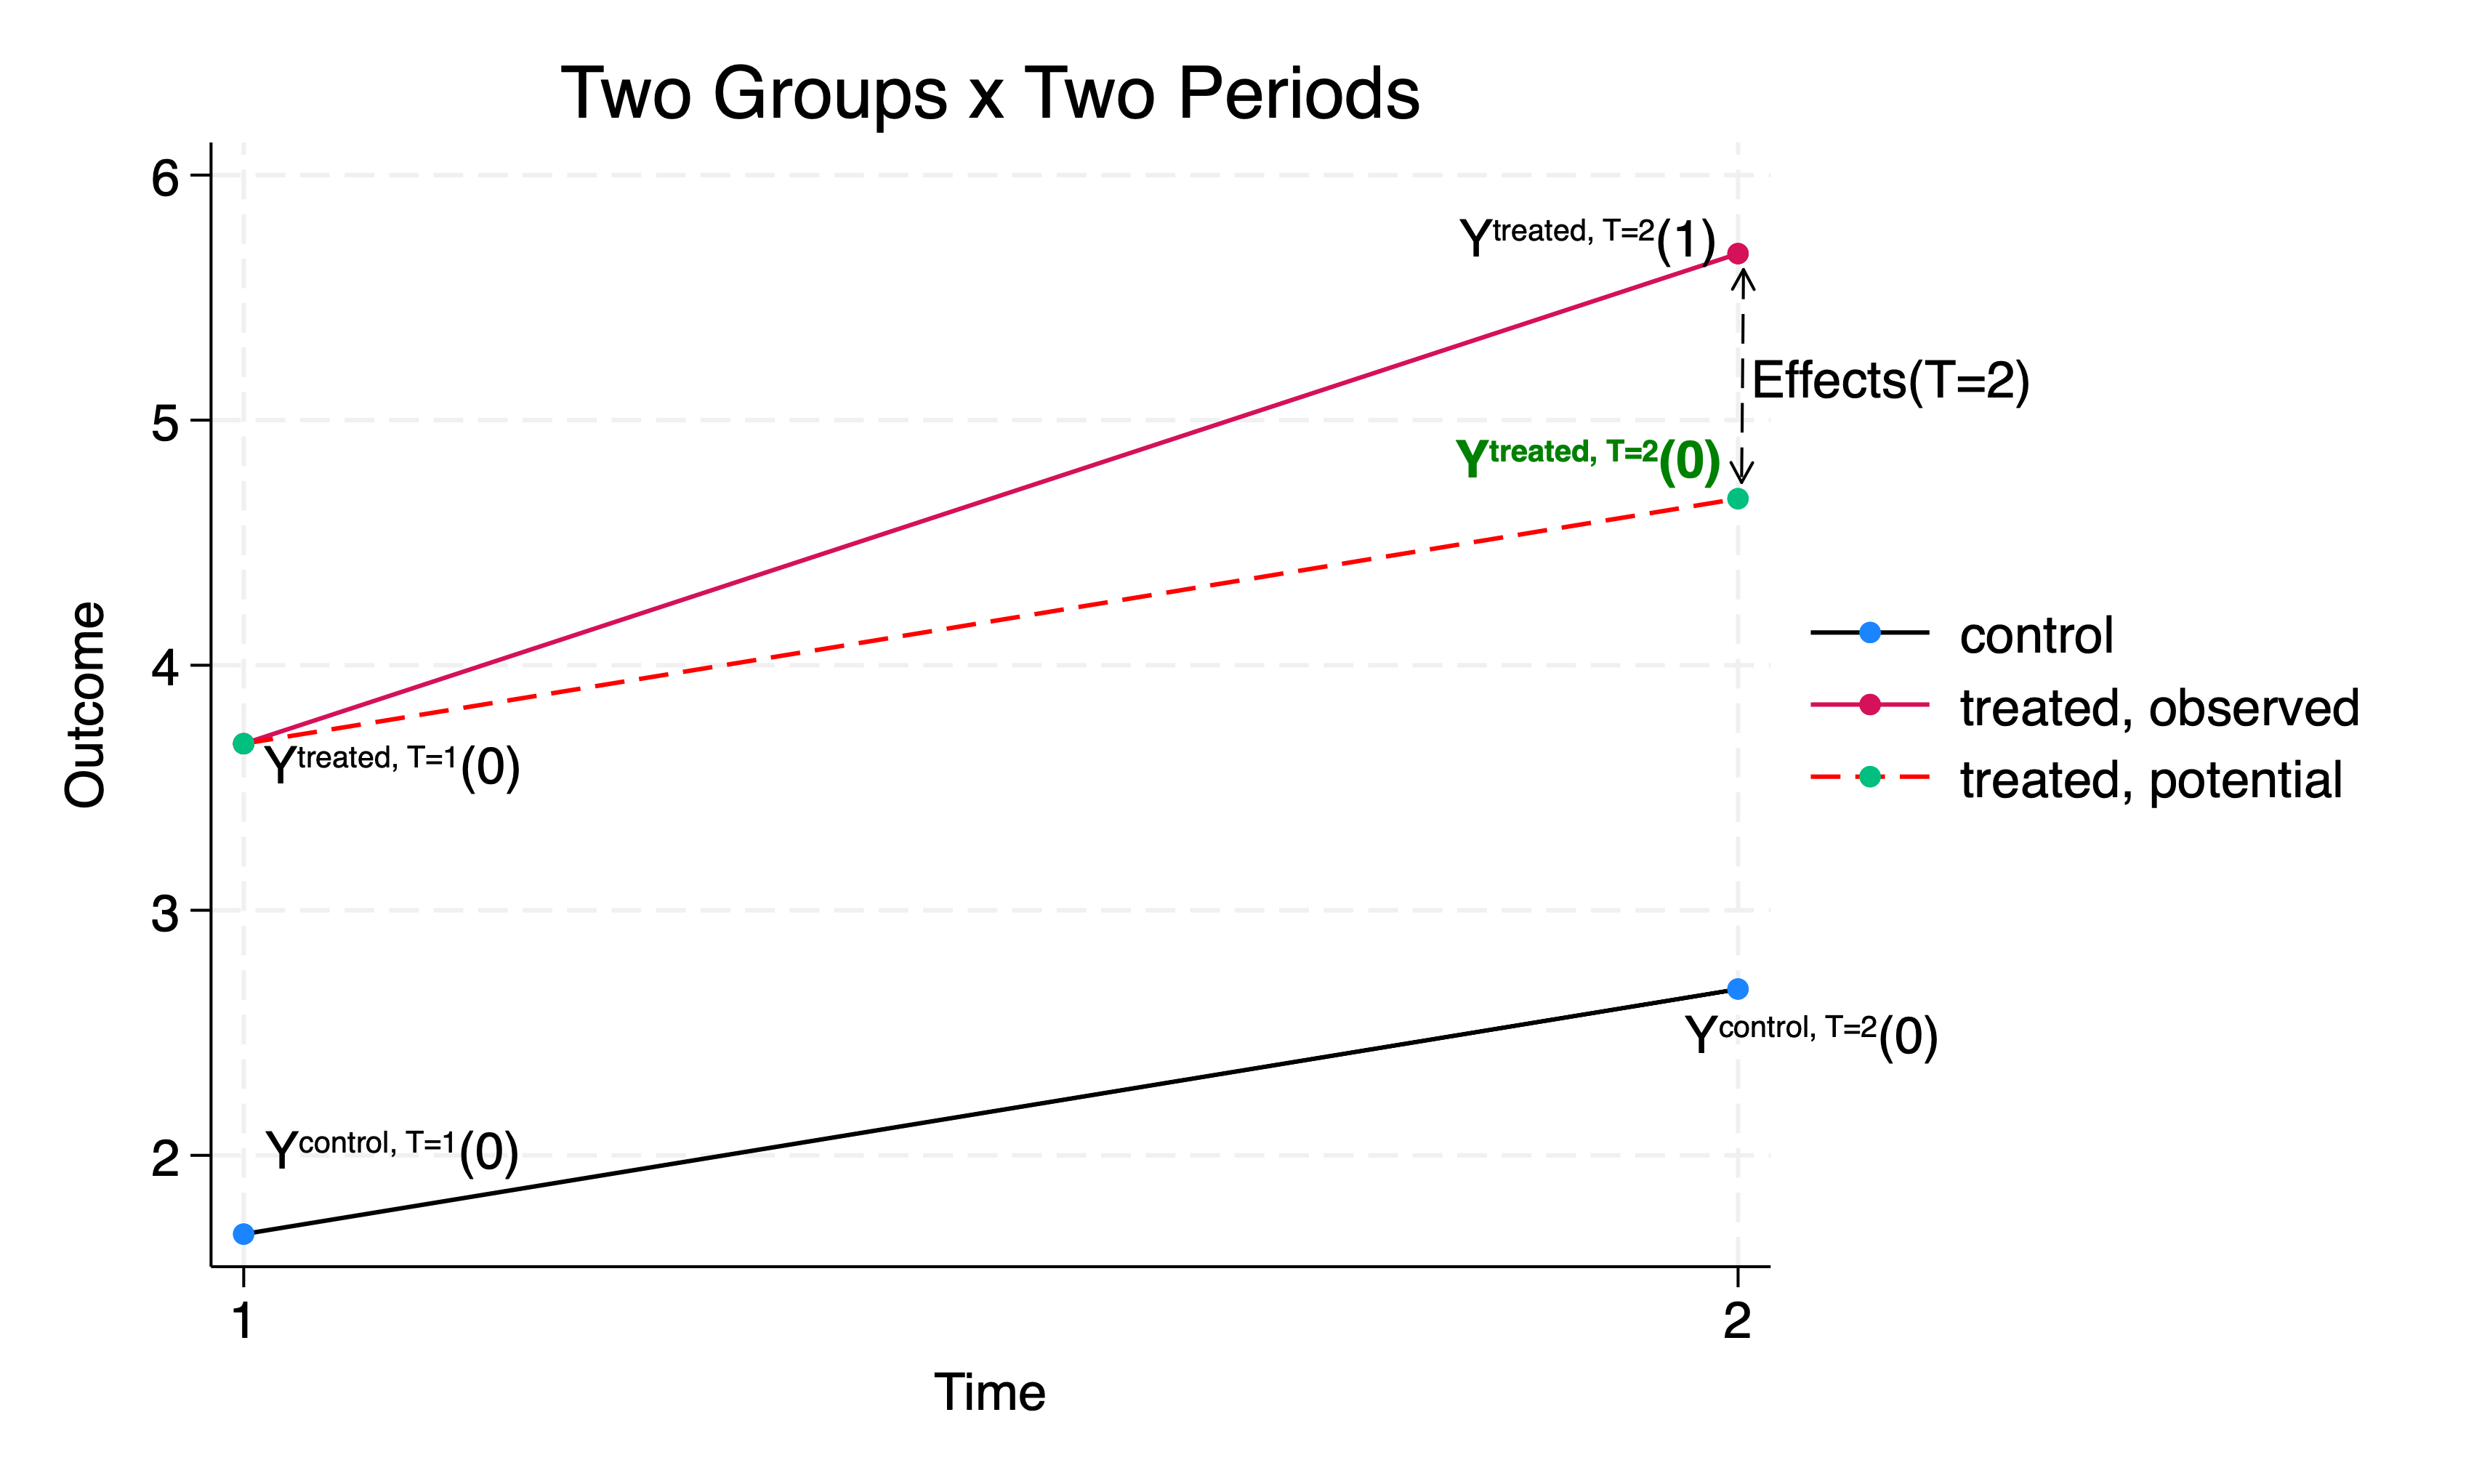
\includegraphics[scale=0.21]{png/did2x2}
\end{figure}
\end{frame}

%------------------------------------------------------------------------------
\begin{frame}
\frametitle{Homogeneous effects across time}
%------------------------------------------------------------------------------
\begin{figure}[H]
\centering
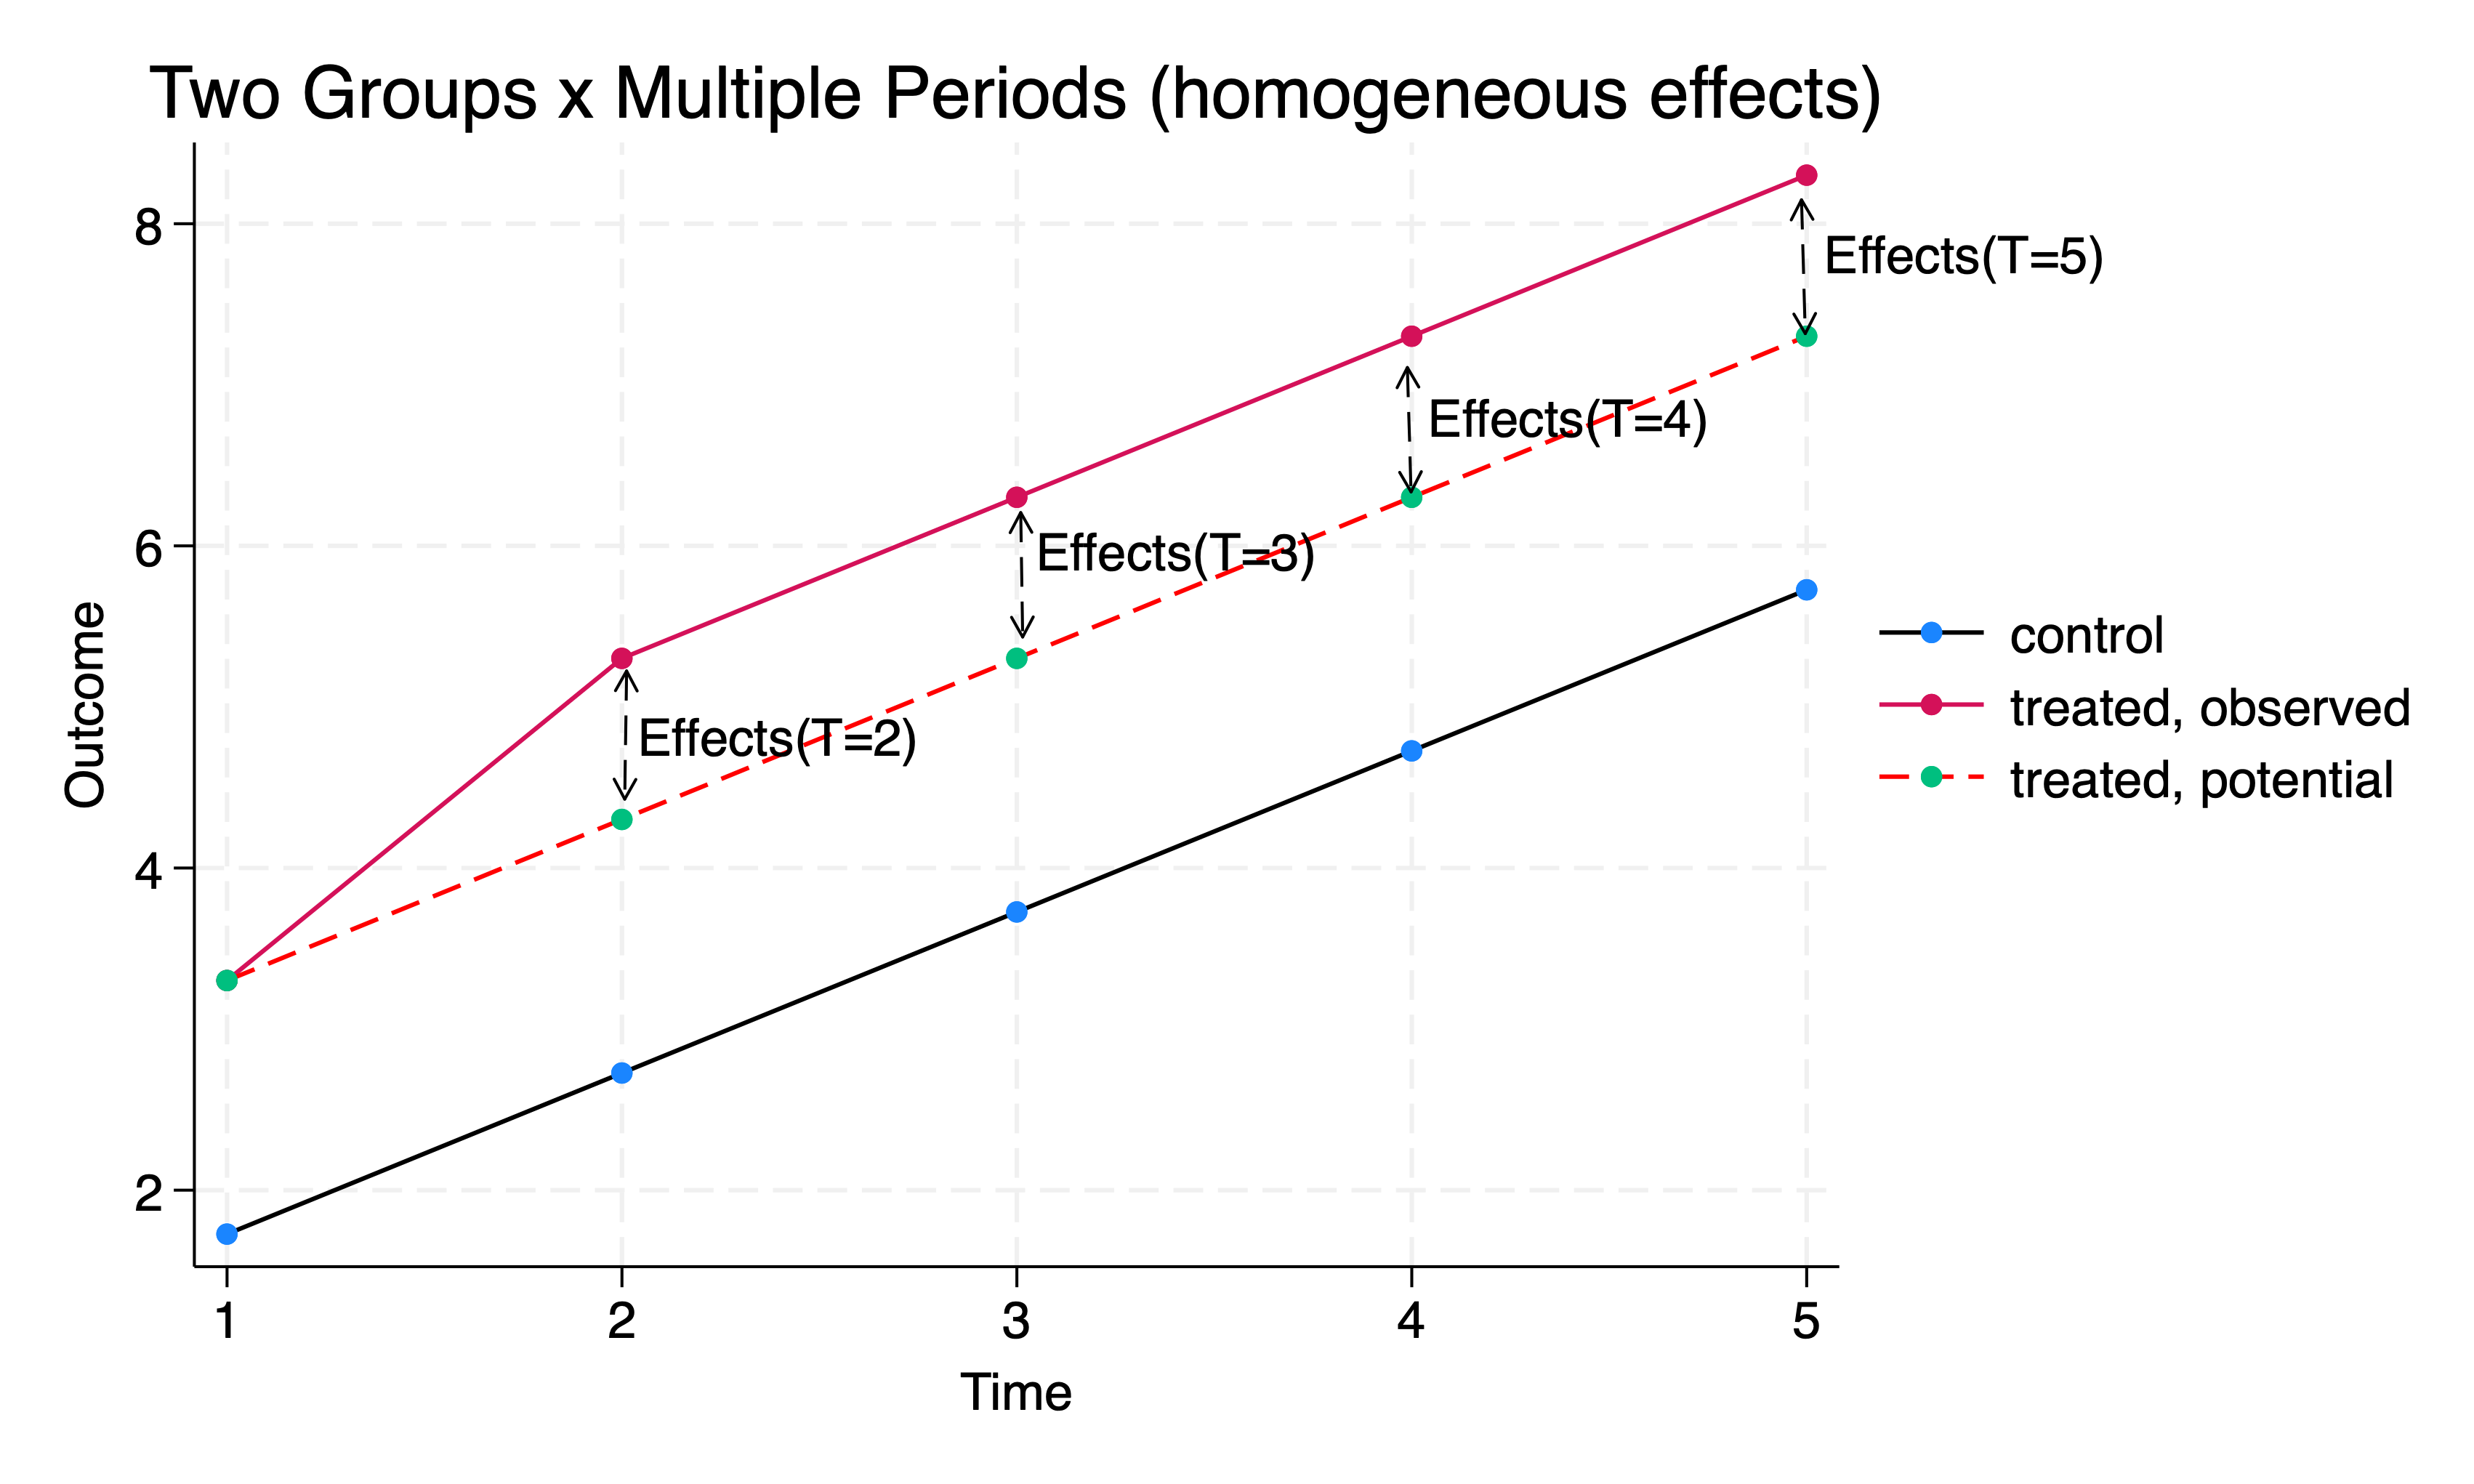
\includegraphics[scale=0.21]{png/did2x5}
\end{figure}
\end{frame}

%------------------------------------------------------------------------------
\begin{frame}
\frametitle{\myred{Heterogeneous} effects across time}
%------------------------------------------------------------------------------
\begin{figure}[H]
\centering
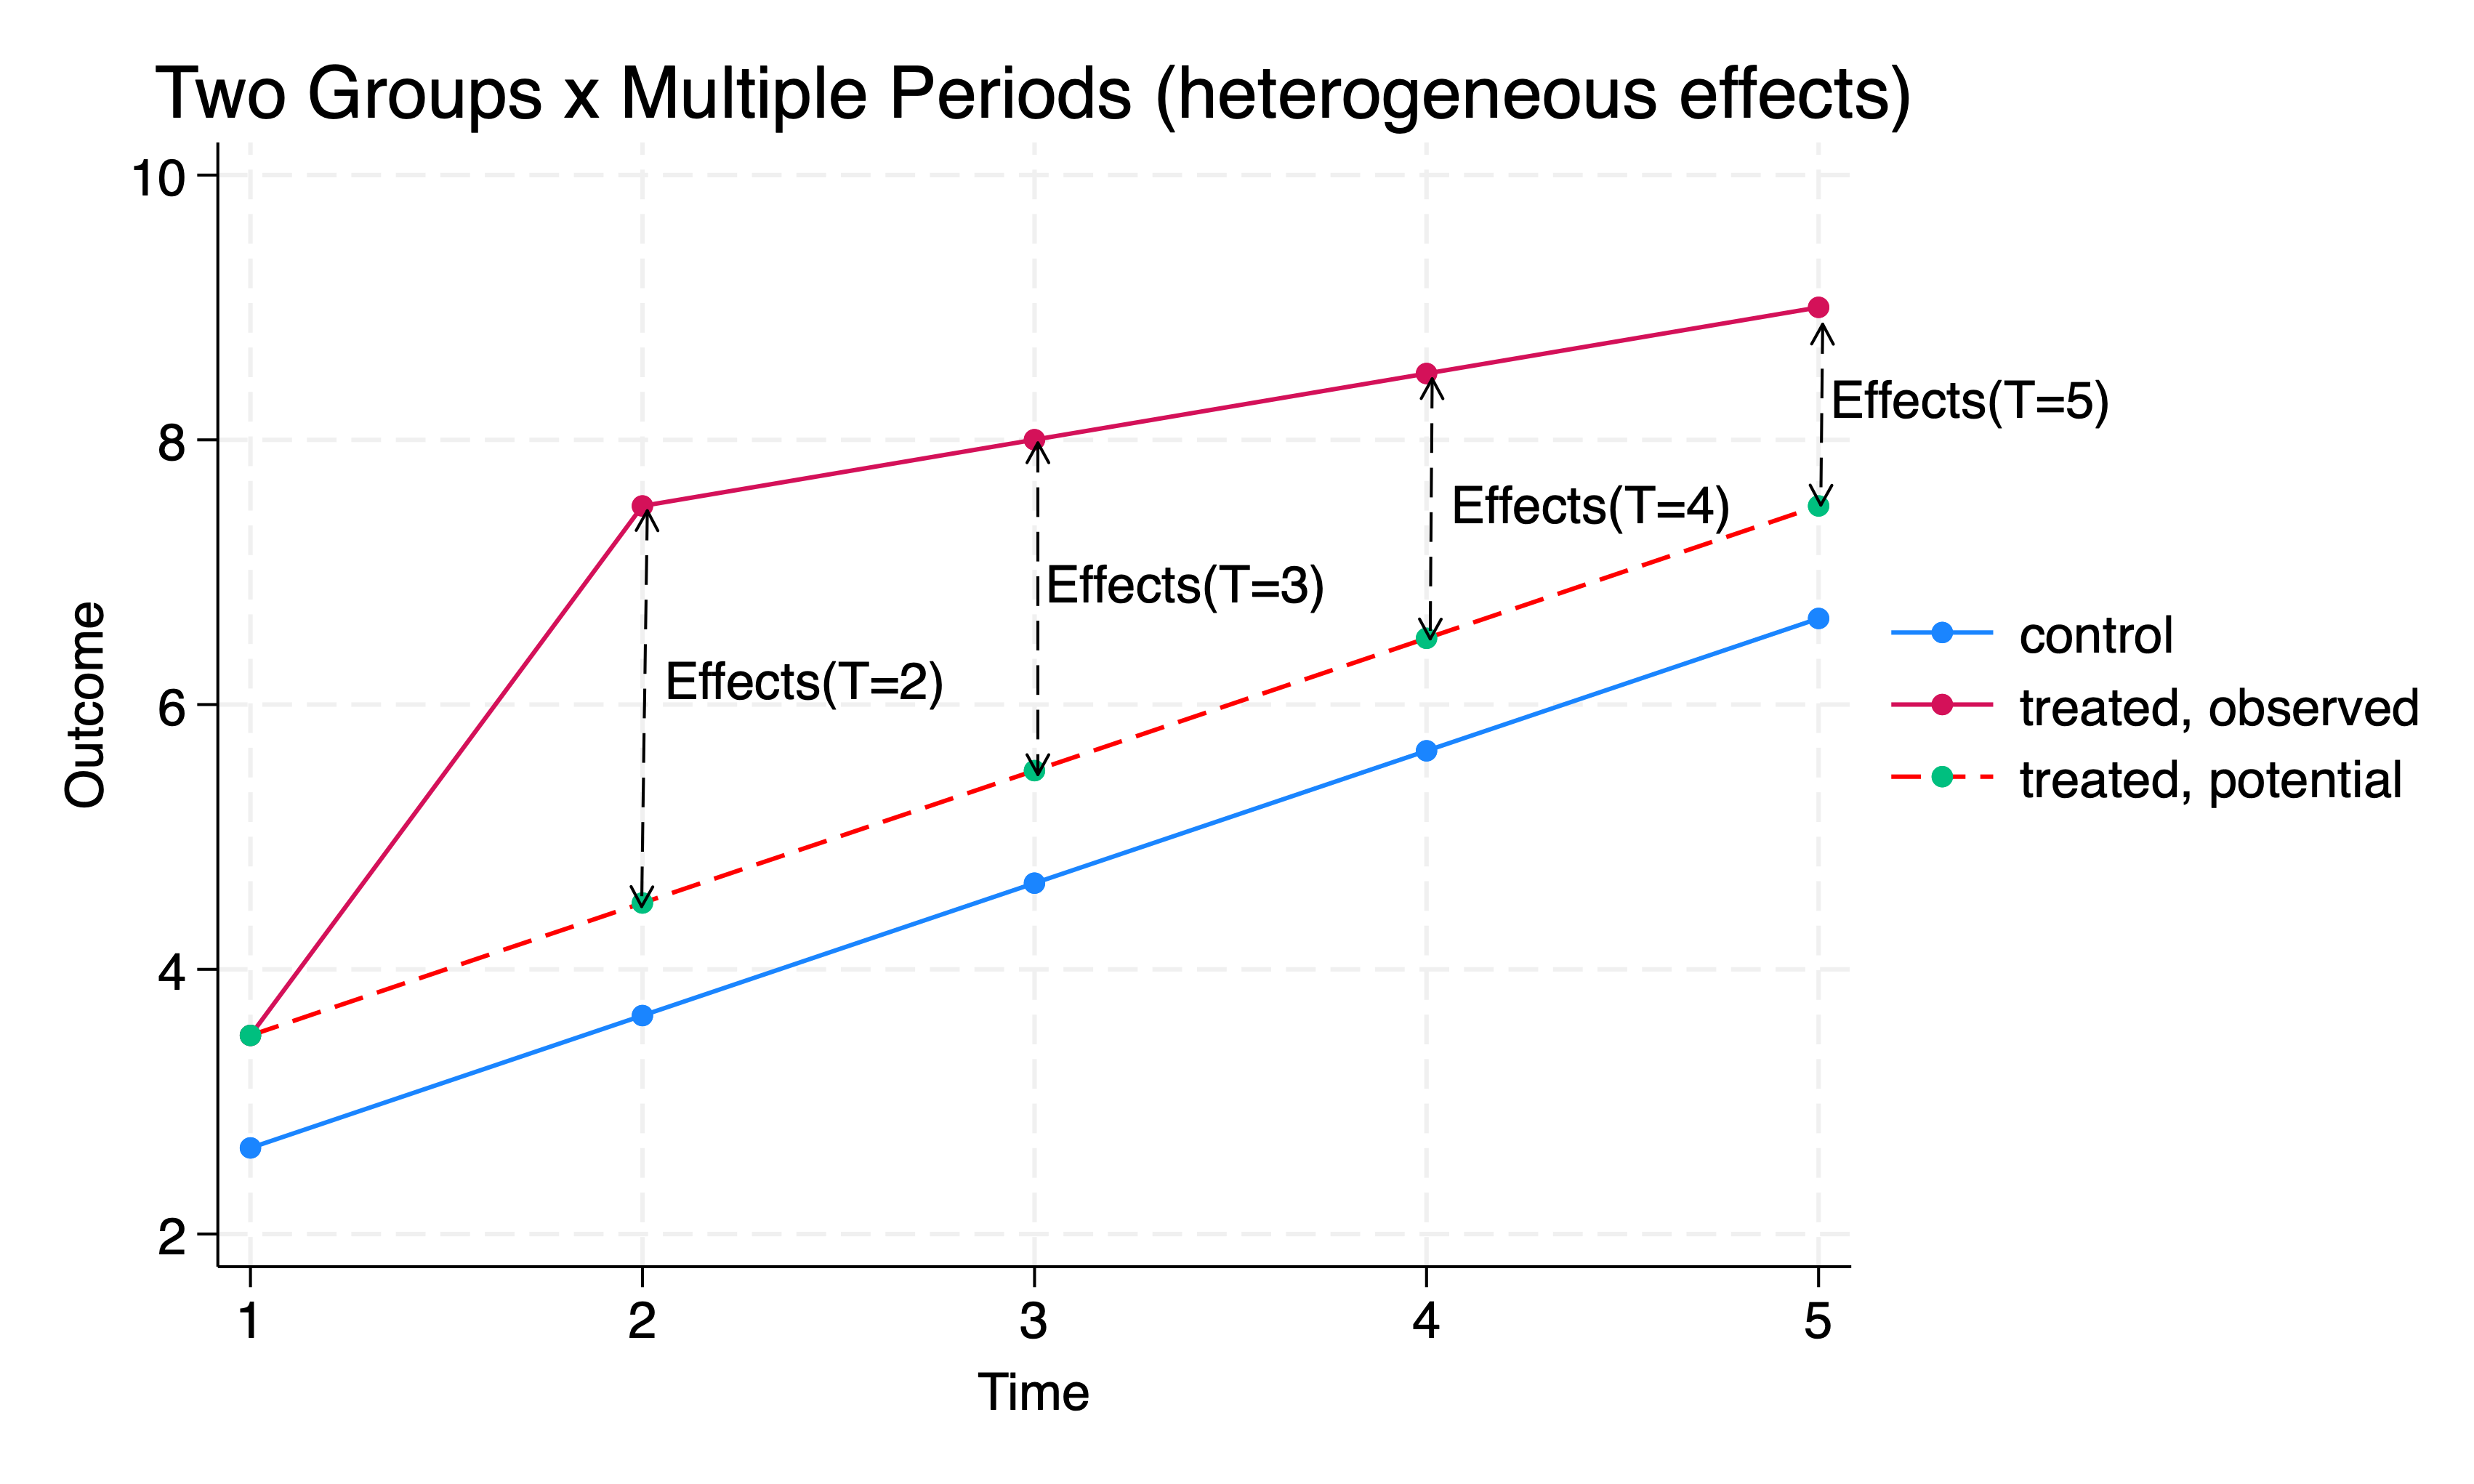
\includegraphics[scale=0.21]{png/did2x5_heter}
\end{figure}
\end{frame}

%------------------------------------------------------------------------------
\begin{frame}
\frametitle{Homogeneous effects across groups and time}
%------------------------------------------------------------------------------
\begin{figure}[H]
\centering
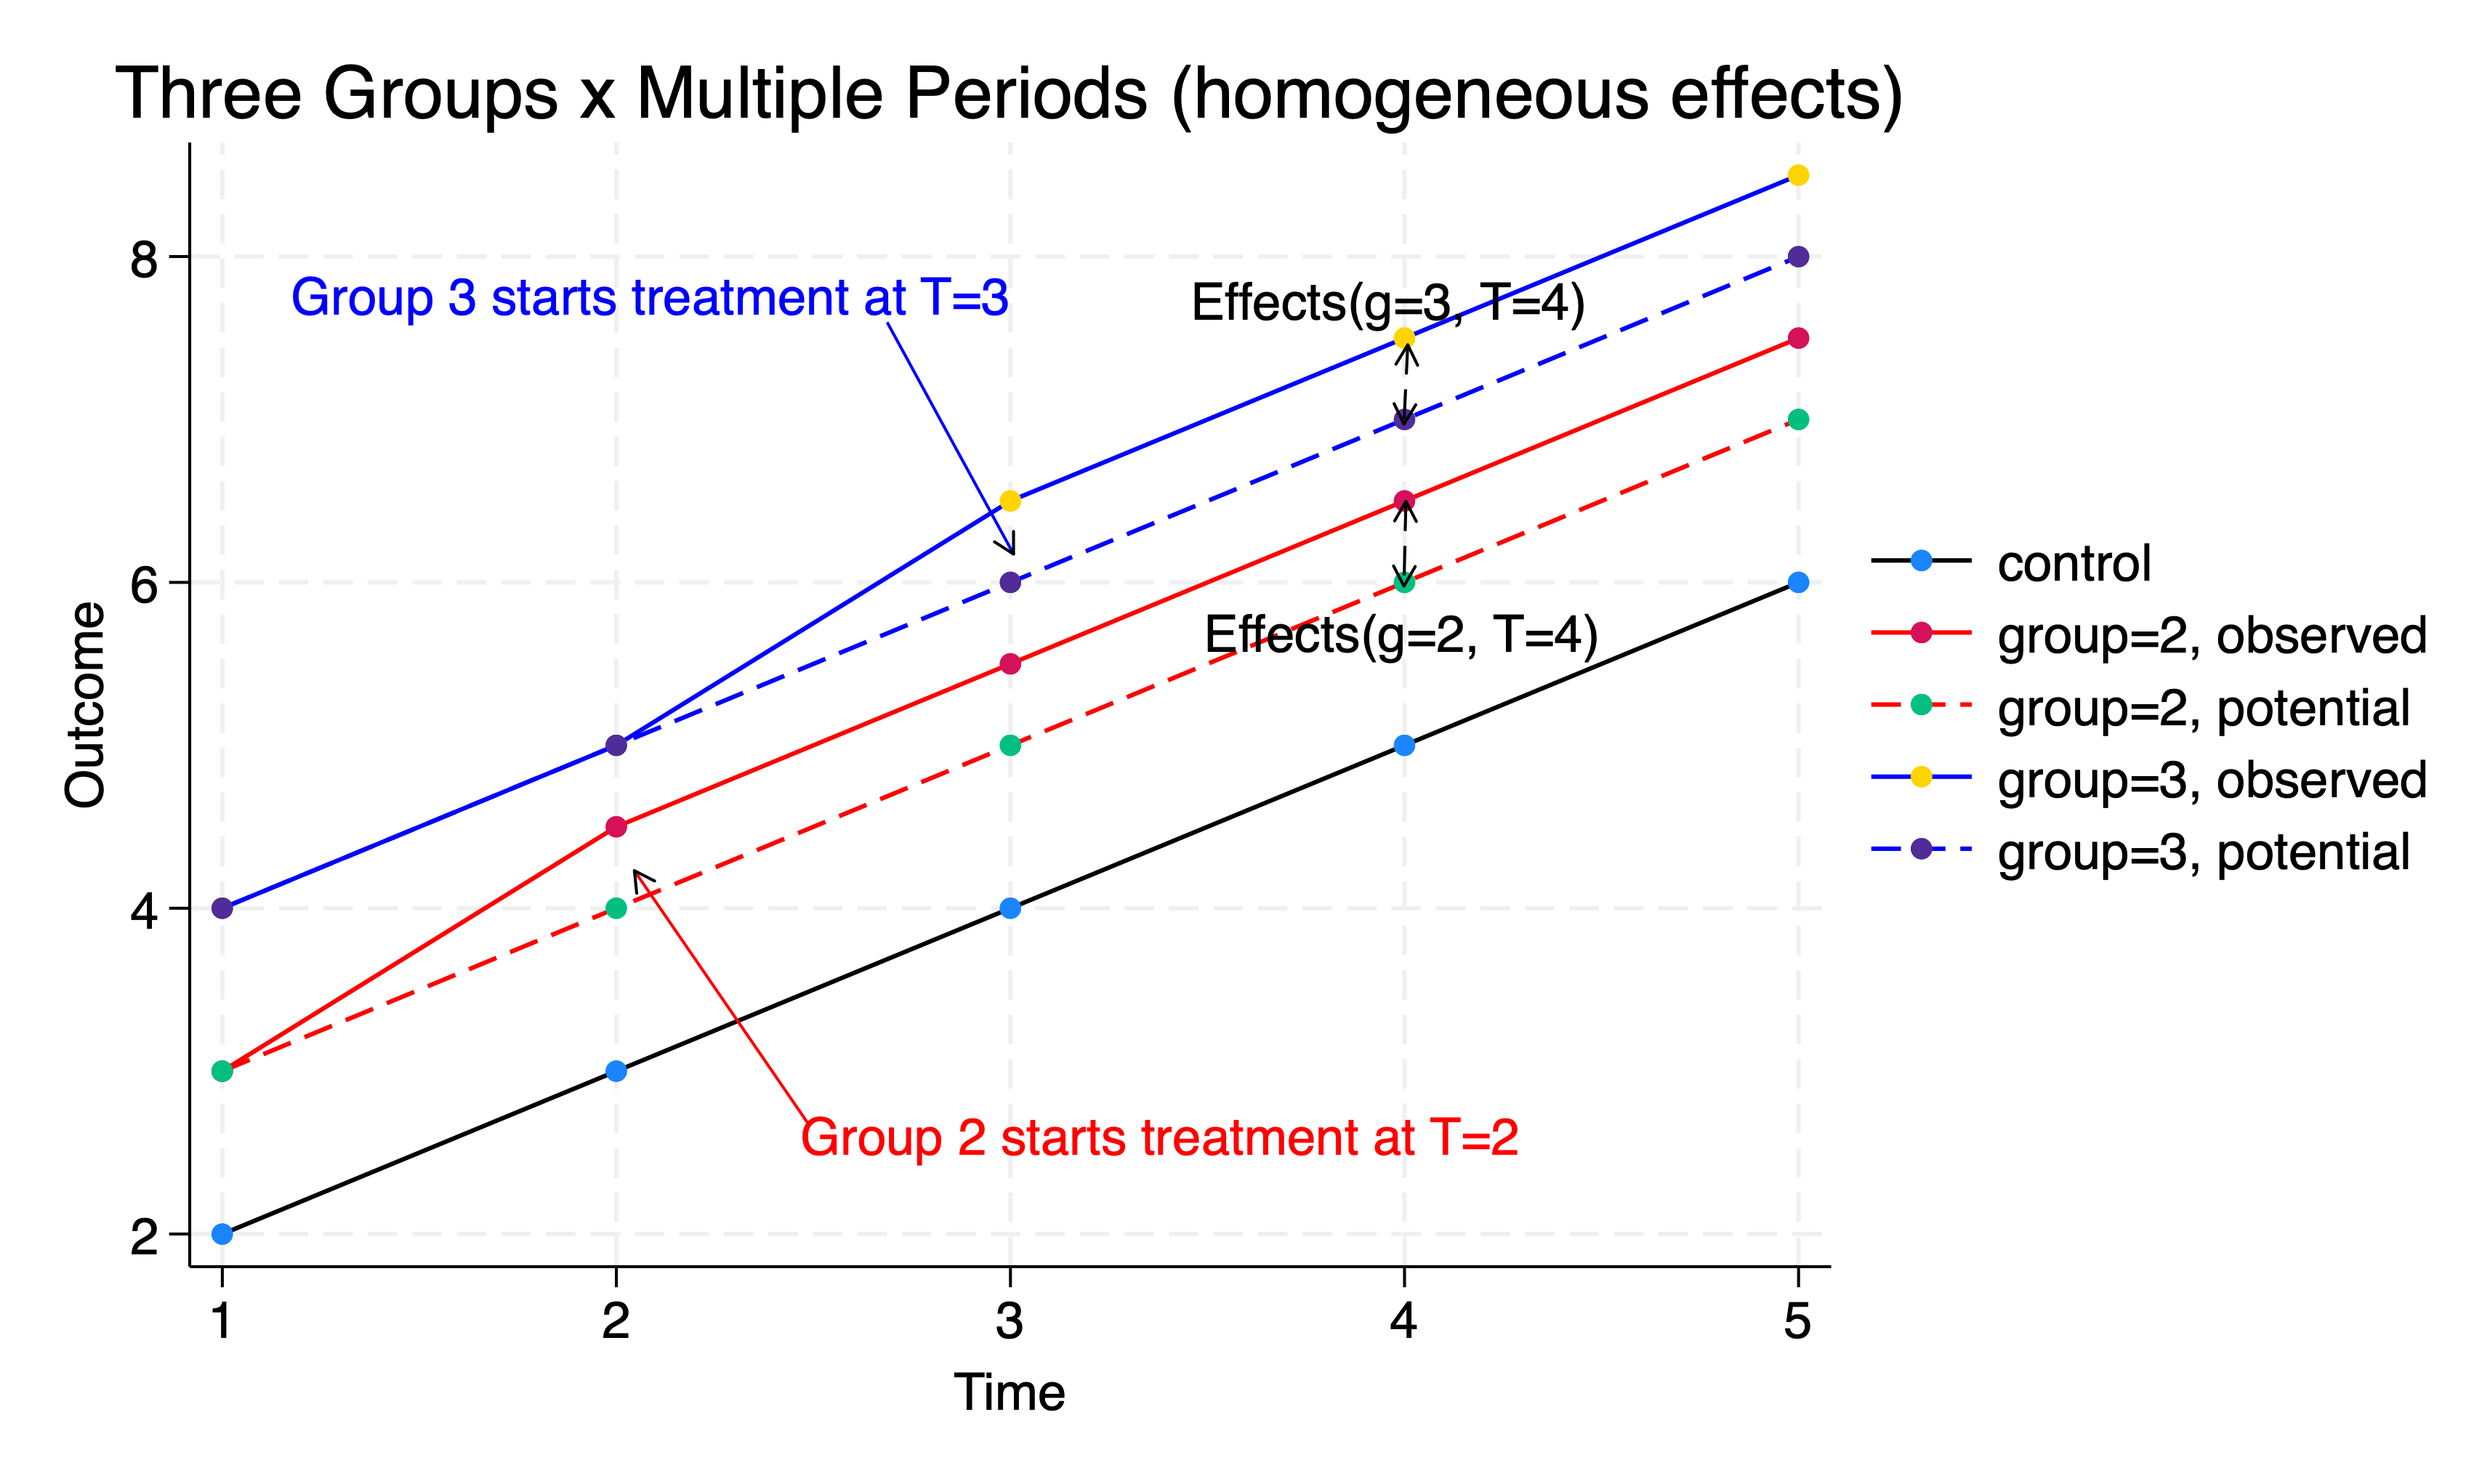
\includegraphics[scale=0.2]{png/did3x5}
\end{figure}
\end{frame}

%------------------------------------------------------------------------------
\begin{frame}
\frametitle{\myred{Heterogeneous} effects across groups and time}
%------------------------------------------------------------------------------
\begin{figure}[H]
\centering
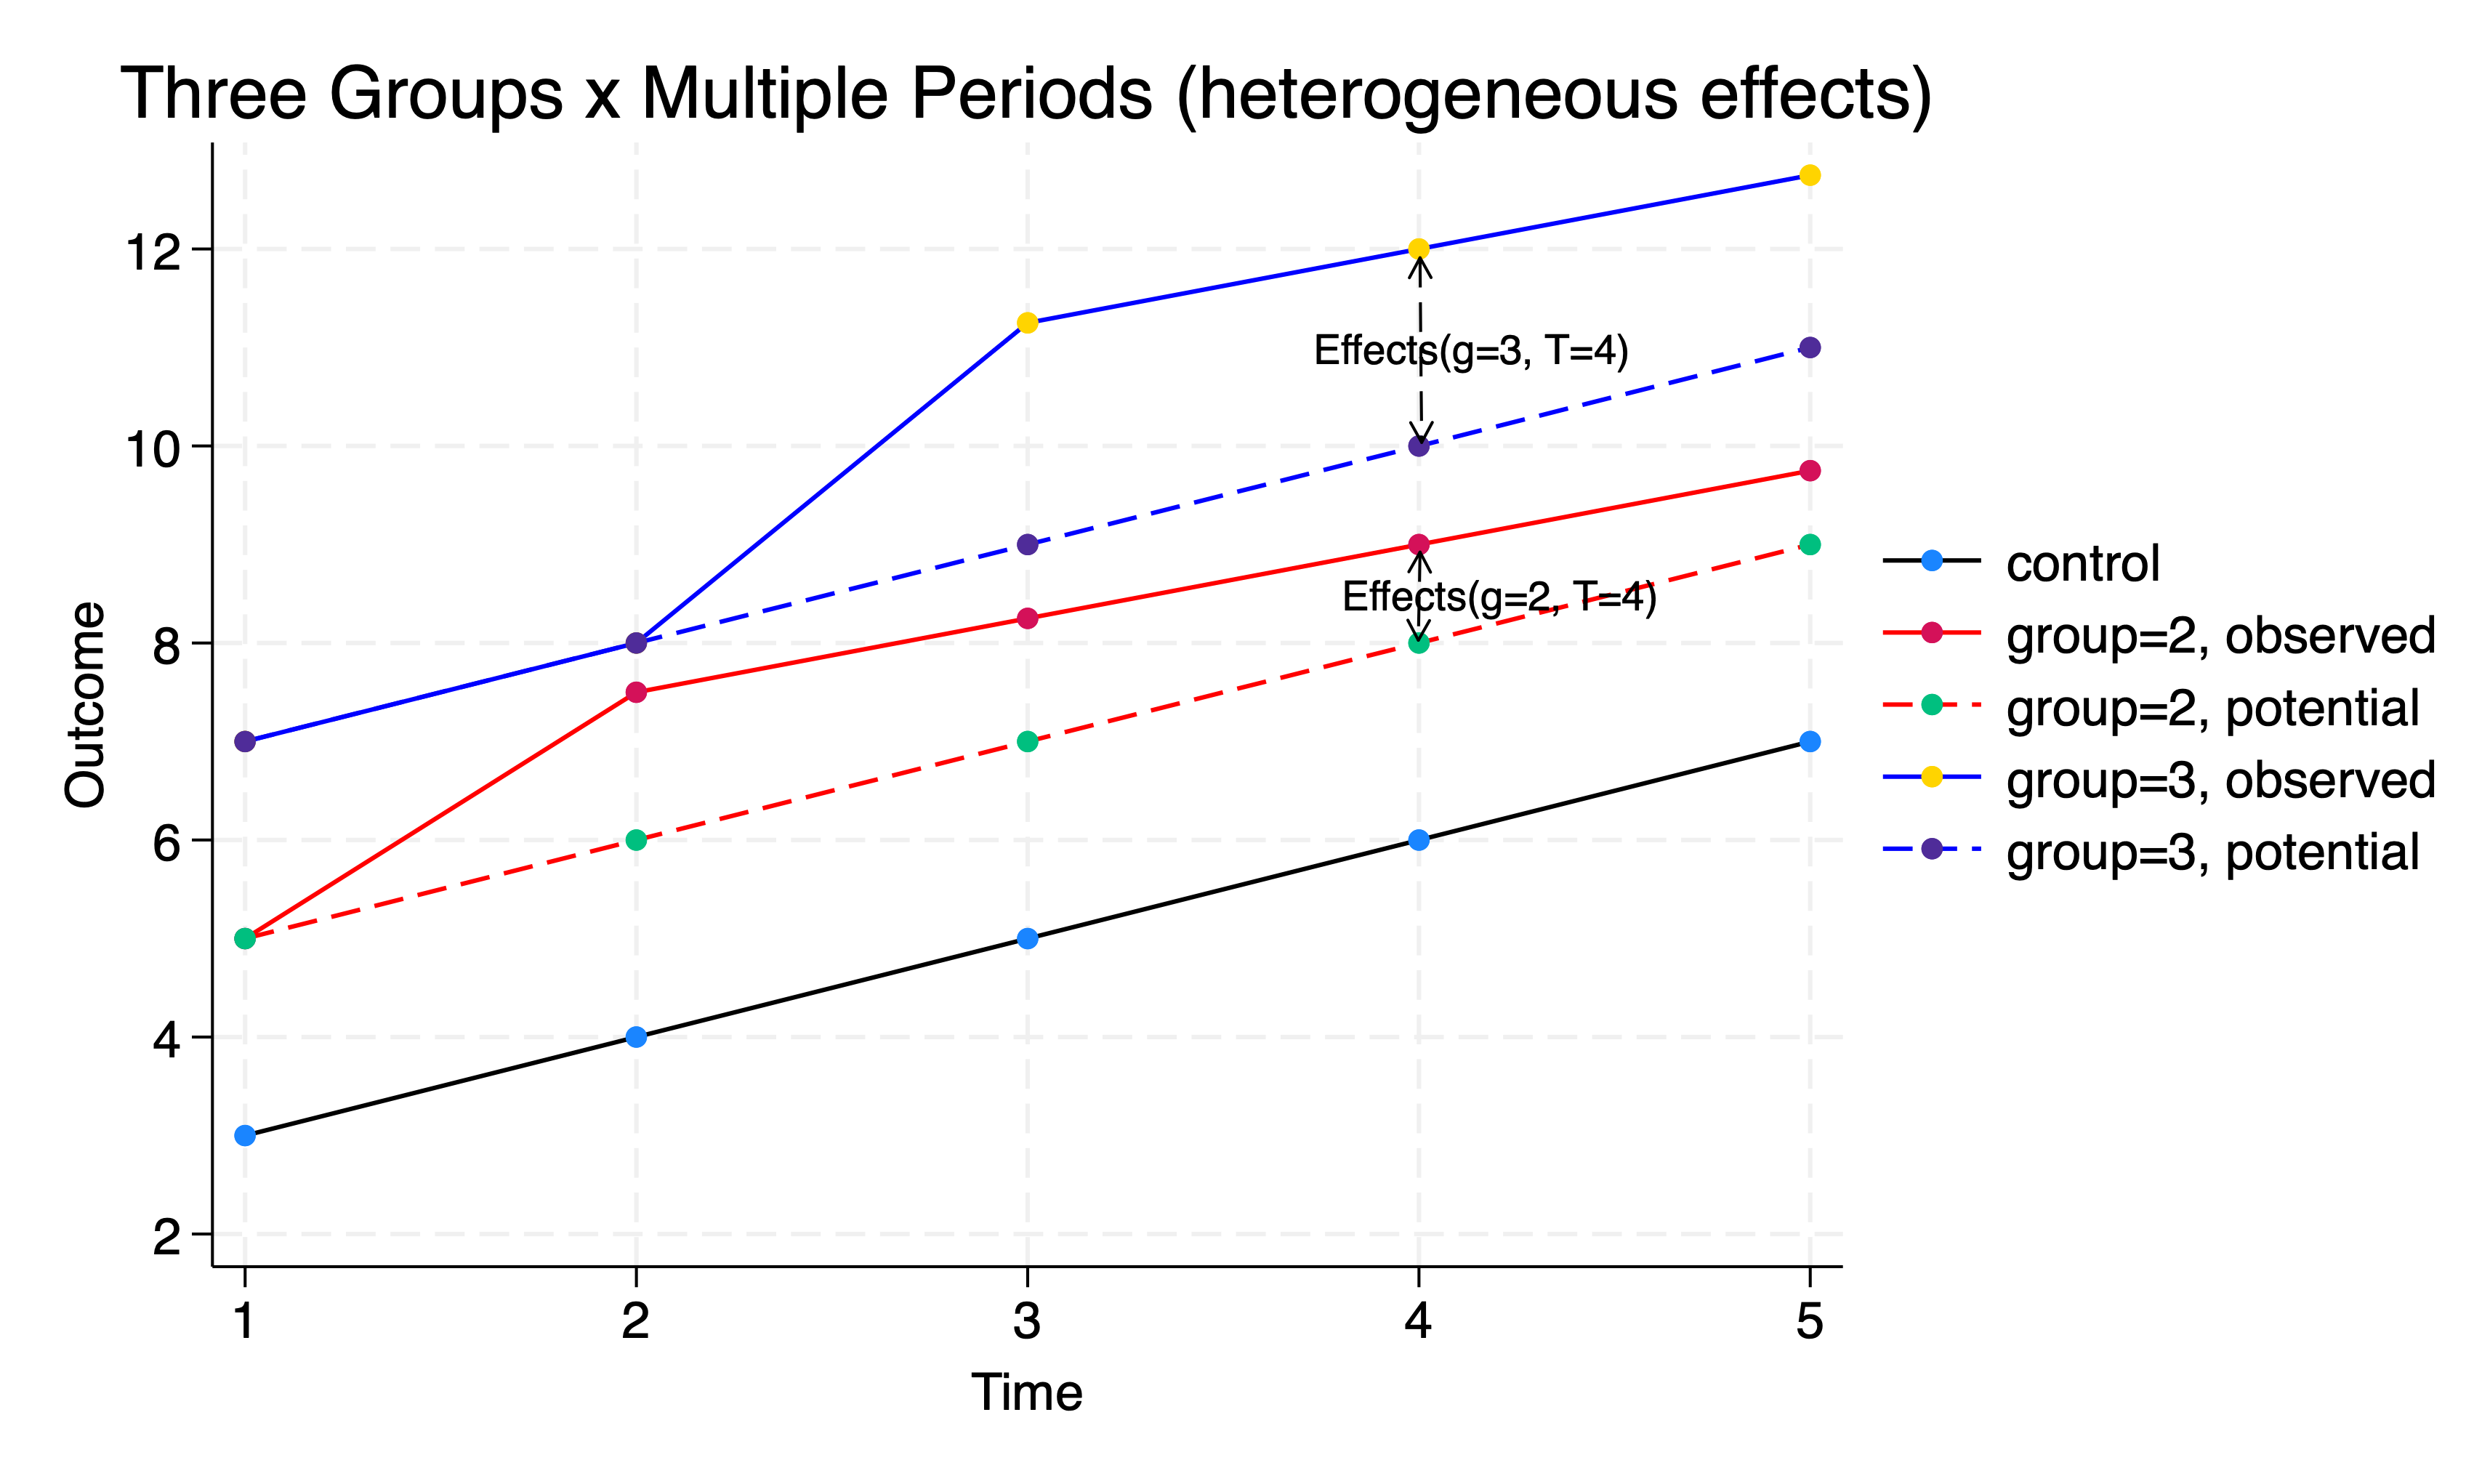
\includegraphics[scale=0.2]{png/did3x5_heter}
\end{figure}
\end{frame}

%%------------------------------------------------------------------------------
\begin{frame}
\frametitle{Problematic TWFE}
%------------------------------------------------------------------------------

$$
y_{it} = \theta_t + \eta_i +  d_{it} \myred{\alpha} + v_{it}
$$

\vskip 1cm

But, 
$$
\alpha = \sum w_k \myblue{Good\_DID}_k + \sum w_j \myred{Bad\_DID}_j
$$

\begin{enumerate}
\item Newly treated relative to the control group (\myblue{good})
\item Newly treated relative to the not-yet treated group (\myblue{good})
\item Newly treated relative to already treated group (\myred{bad})
\end{enumerate}
\end{frame}

%------------------------------------------------------------------------------
\begin{frame}
\frametitle{When is TWFE good?}
%------------------------------------------------------------------------------

\begin{enumerate}
\item There are \myred{only two periods}
\item The treatment effects are \myred{homogenenous across both groups and time}
\end{enumerate}

\end{frame}

%------------------------------------------------------------------------------
\begin{frame}
  \frametitle{Overview of heterogeneous DID in Stata 18}
%------------------------------------------------------------------------------
{\bf Estimation}:
\begin{enumerate}
  \item \myred{\tt xthdidregress} and \myred{\tt hdidregress} for panel data and
    repeated cross-section data
  \item Four estimators: \myred{\tt ra}, \myred{\tt ipw}, \myred{\tt aipw} in
\cite{Callaway2021} and \myred{\tt twfe} in \cite{Wooldridge2021}
\end{enumerate}

\vskip 0.3cm
{\bf Post-estimation}:
\begin{enumerate}
  \item \myred{\tt estat atetplot}: visualize ATETs
  \item \myred{\tt estat aggregation}: aggregate ATETs along different
    dimensions
  \item \myred{\tt estat ptrends}: pre-treatment parallel trend tests
  \item \myred{\tt estat sci}: simultaneous CI for RA, IPW, and AIPW estimators
\end{enumerate}
\end{frame}

%------------------------------------------------------------------------------
\section{Example: minimum wage}
\begin{frame}
  \frametitle{Increasing minimum wage and young employment}
%------------------------------------------------------------------------------
  \vskip 0.5cm

\begin{itemize}
    \setlength\itemsep{0.5em}
  \item {\bf Outcome}: county-level employment for young workers
  \item {\bf Treatment}: minimum wage restrictions introduced by State
    government; see \cite{Callaway2021} 
  \item {\bf Multiple periods}: 2002 - 2007 (6 years)
  \item {\bf Multiple treatment timings}: 2004, 2006, 2007
\end{itemize}

\end{frame}

%------------------------------------------------------------------------------
\begin{frame}
  \frametitle{{\tt xthdidregress aipw}}
%------------------------------------------------------------------------------
 
{\bf Define covariates}

    \vskip 0.2cm
{\footnotesize \tt 
global covars i.region pop medinc white hs pov ///
}

\hskip 1.3cm
{\footnotesize \tt 
    c.pop\#c.pop c.medinc\#c.medinc
}

\vskip 0.5cm
{\bf Use AIPW estimator}

    \vskip 0.2cm
\hyperlink{hdid_output.pdf.2}{\footnotesize \tt
  xthdidregress aipw (lemp \$covars) (treat \$covars), group(state)
}

\begin{itemize}
  \item Adding covariates for conditional parallel trend 
  \item There are $18$ ATET(g,t)'s (6 years $\times$ 3 cohorts)
  \item Standard errors are adjusted by clusters of state
\end{itemize}
\end{frame}

%------------------------------------------------------------------------------
\begin{frame}
  \frametitle{{\tt estat atetplot, sci}}
%------------------------------------------------------------------------------
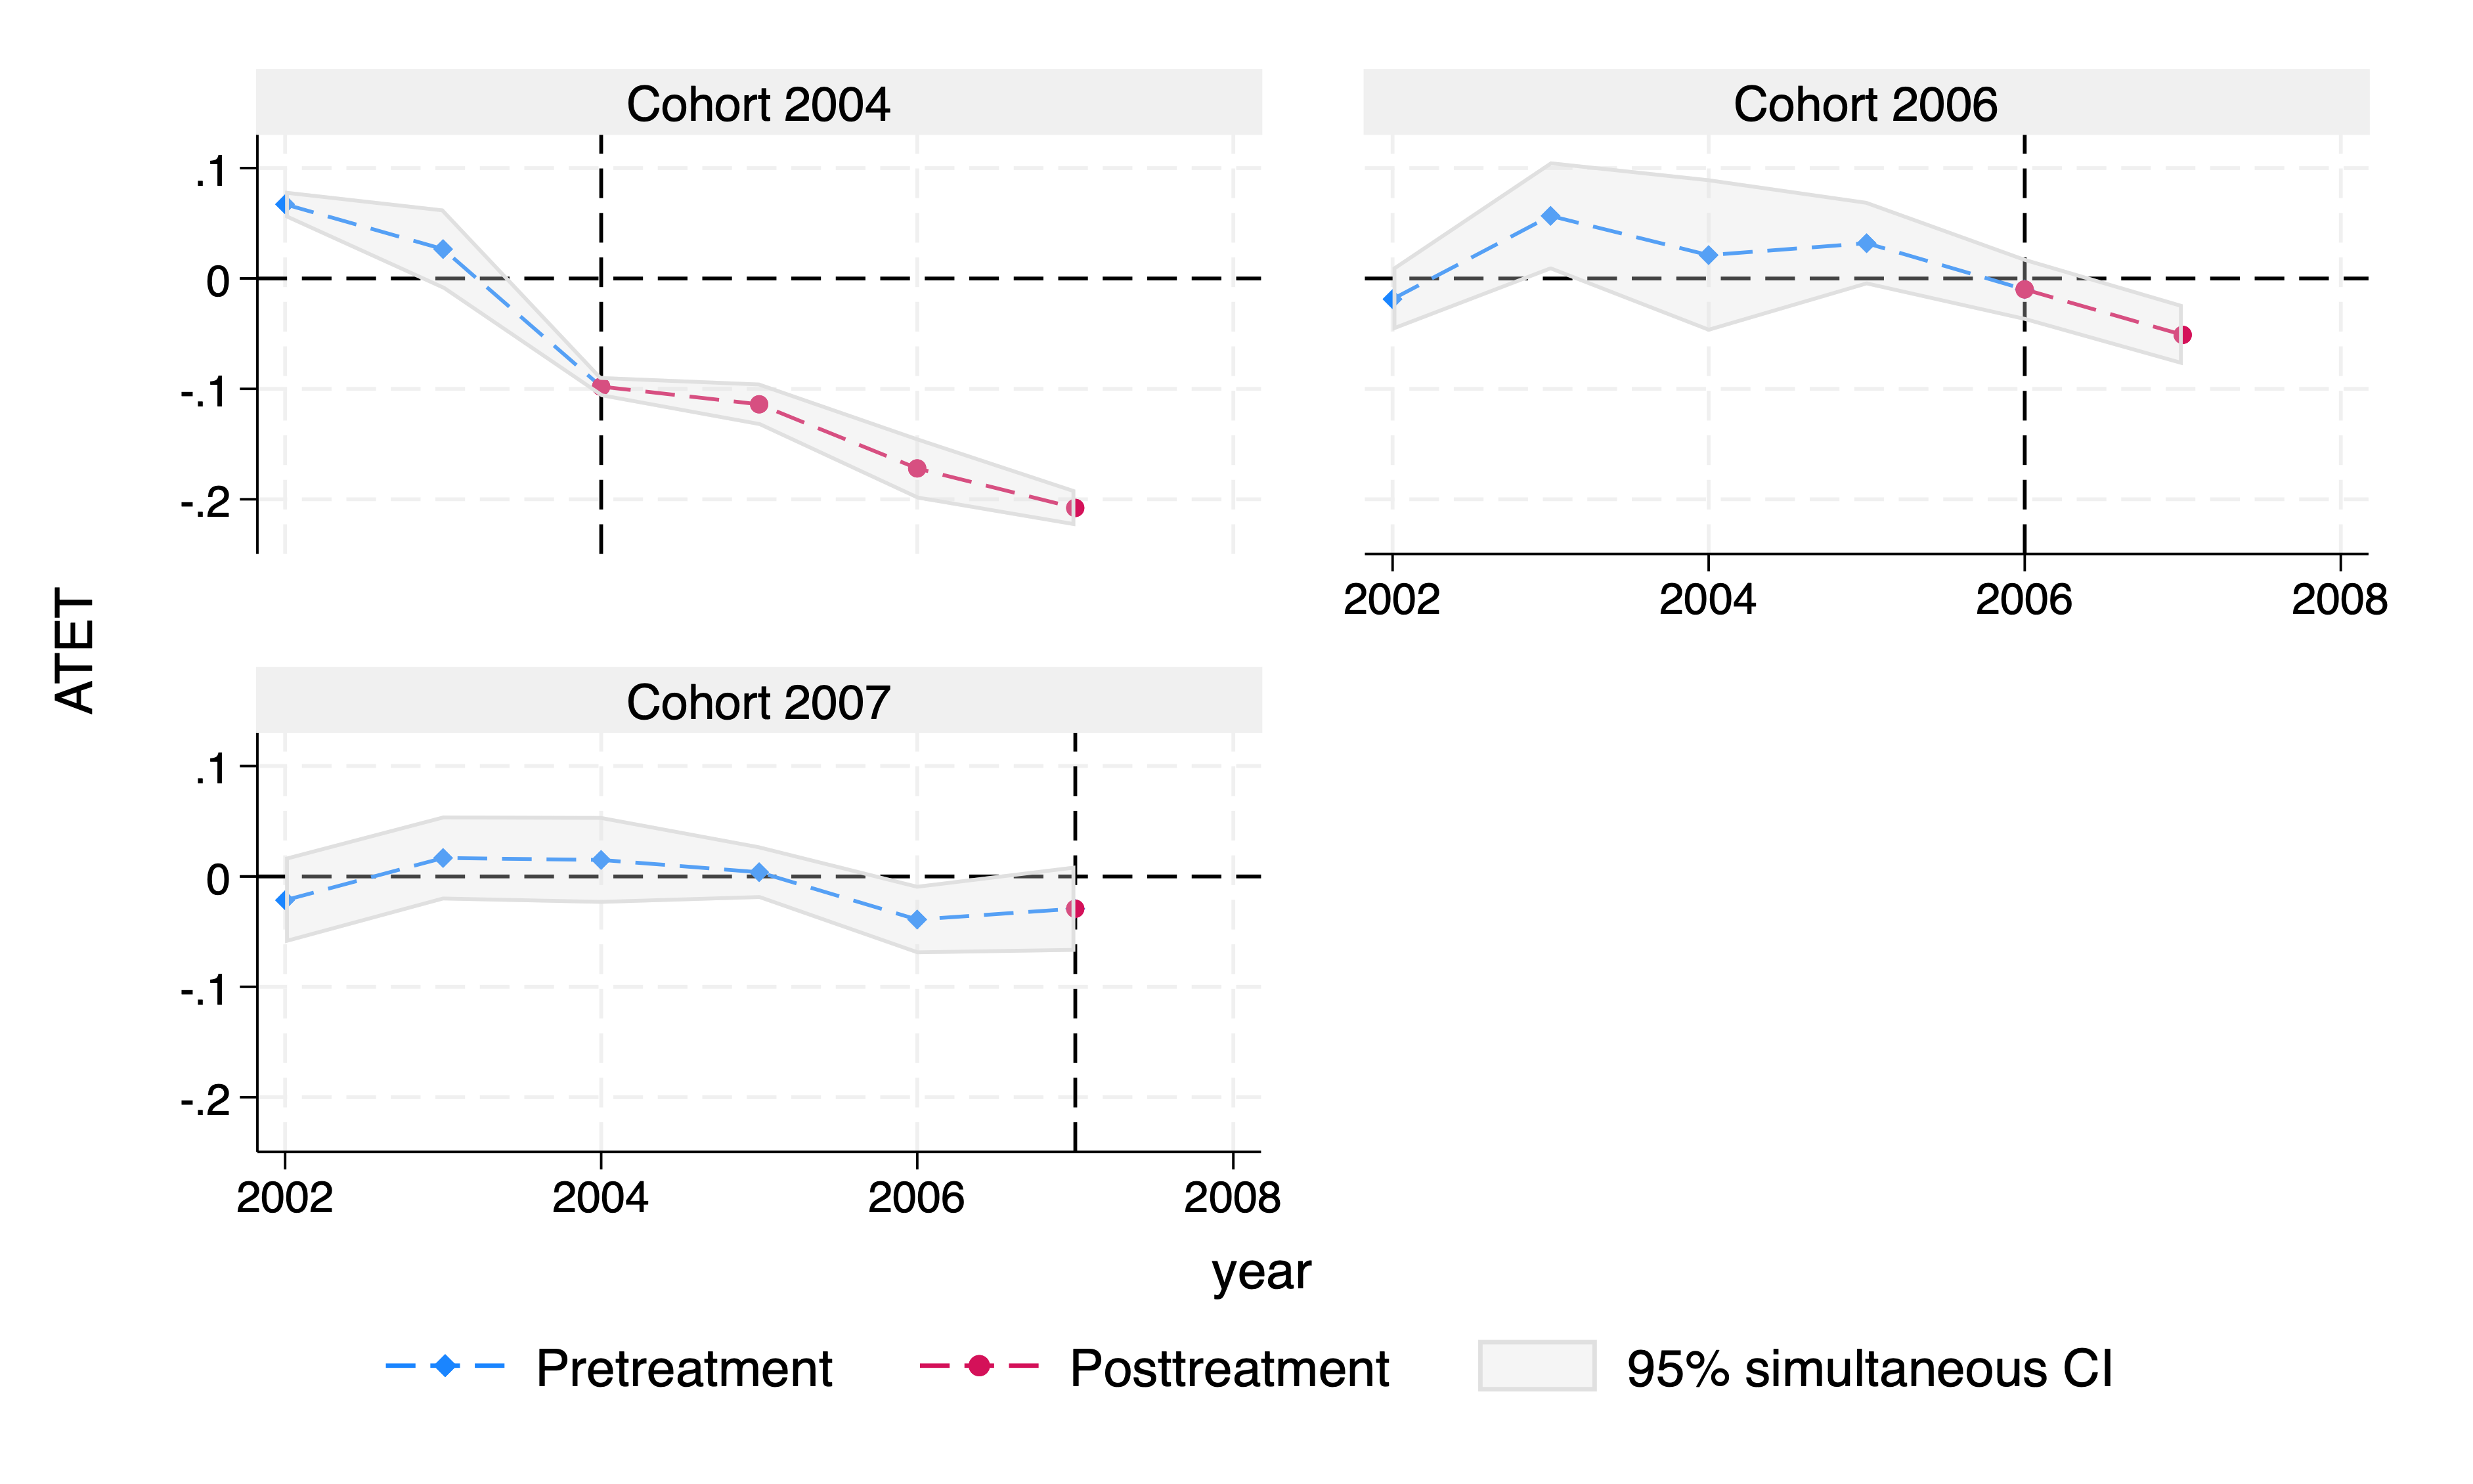
\includegraphics[scale=0.15]{png/g2}

\begin{itemize}

  \item Specify option \myred{\tt sci} for simultaneous confidence intervals

  \item For cohorts 2004 and 2006, minimum wage restriction decreases the
    employment rate for young workers
\end{itemize}
\end{frame}

%------------------------------------------------------------------------------
\section{Aggregate ATET's}
\begin{frame}
  \frametitle{Summarize ATET(g,t)'s}
%------------------------------------------------------------------------------
\begin{itemize}
  \item How do the ATETs vary with the length of \myred{exposure to the
    treatment}? (event study)
  
  \item How do the ATETs vary with \myred{cohorts}? (does start treatment
    earlier matter?)

  \item How do the ATETs vary with \myred{time}? (Good year vs. lousy year)

  \item Overall ATETs across time and cohorts
\end{itemize}

\vskip 0.3cm
We can express the aggregations as a weighted mean of all ATETs
$$
\theta = \sum_{g \in \G} \sum_{t=2}^T 
\myred{\underbrace{w(g,t)}_\text{weight}}
\myblue{ATET(g,t)}
$$

\end{frame}

%------------------------------------------------------------------------------
\begin{frame}
  \frametitle{Event study}
%------------------------------------------------------------------------------
  \begin{itemize}
    \item
Let $e = t - g$ be the length of exposure to the treatment. 
\begin{align*}
  \theta(\myred{\bf e}) = \sum_{g\in\G} 
  \myred{\underbrace{\I(g + e \leq T) \Pr(G=g | G + e \leq T)}_\text{propotions
  used to estimate ATET(g, g+e)}}
  ATET(g, g+e)
\end{align*}

\item
  \hyperlink{hdid_output.pdf.3}{\tt estat aggregation, weights(cohort)
  {\bf dynamic}
 \myred{graph}}
\end{itemize}
\begin{figure}[H]
\centering
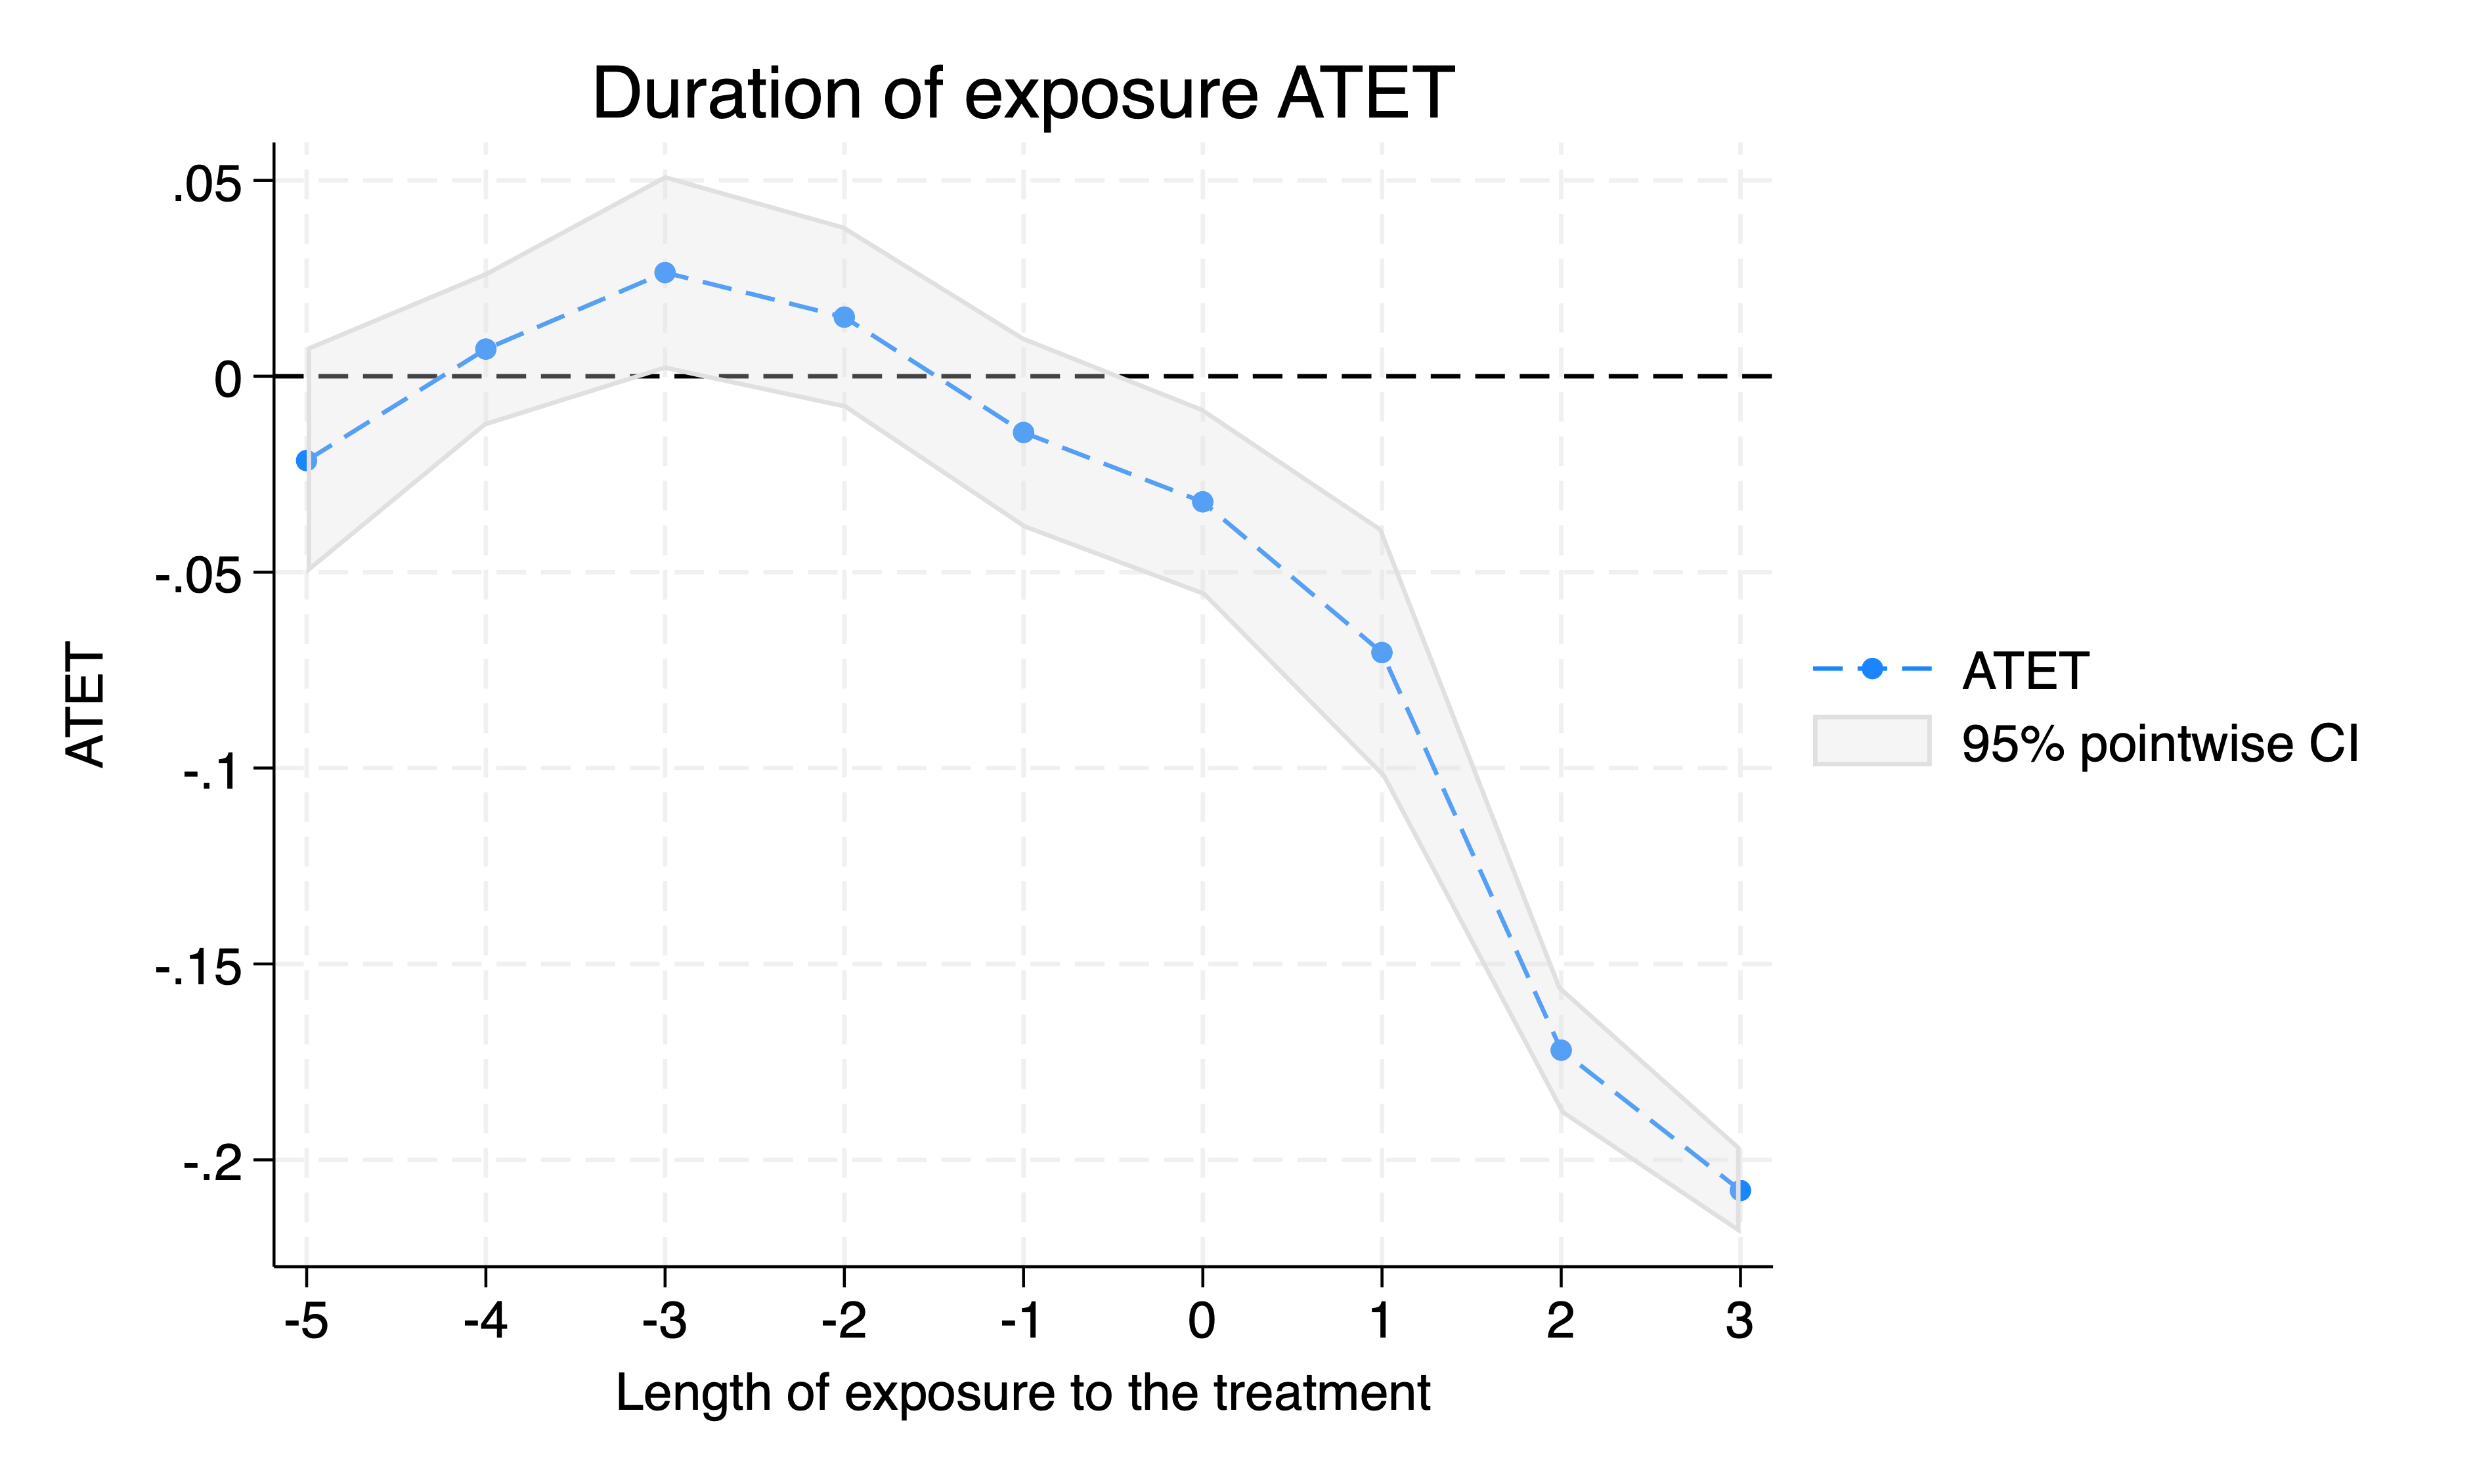
\includegraphics[scale=0.12]{png/d2}
\end{figure}
\end{frame}

%------------------------------------------------------------------------------
\begin{frame}
  \frametitle{ATETs over cohort}
%------------------------------------------------------------------------------
\begin{align*}
  \theta(\myred{\bf g}) = \sum_{t=g}^T \myred{\underbrace{
  \frac{1}{T - g +1} \I(t \geq g)
  }_\text{proportions used to estimate post-treatment ATET(g,t)}}
  ATET(g, t)
\end{align*}

\vskip 0.3cm
\begin{itemize}
\item 
\hyperlink{hdid_output.pdf.3}{\tt estat aggregation, weights(cohort) 
{\bf cohort}
 \myred{graph}}

 \end{itemize}

\begin{figure}[H]
\centering
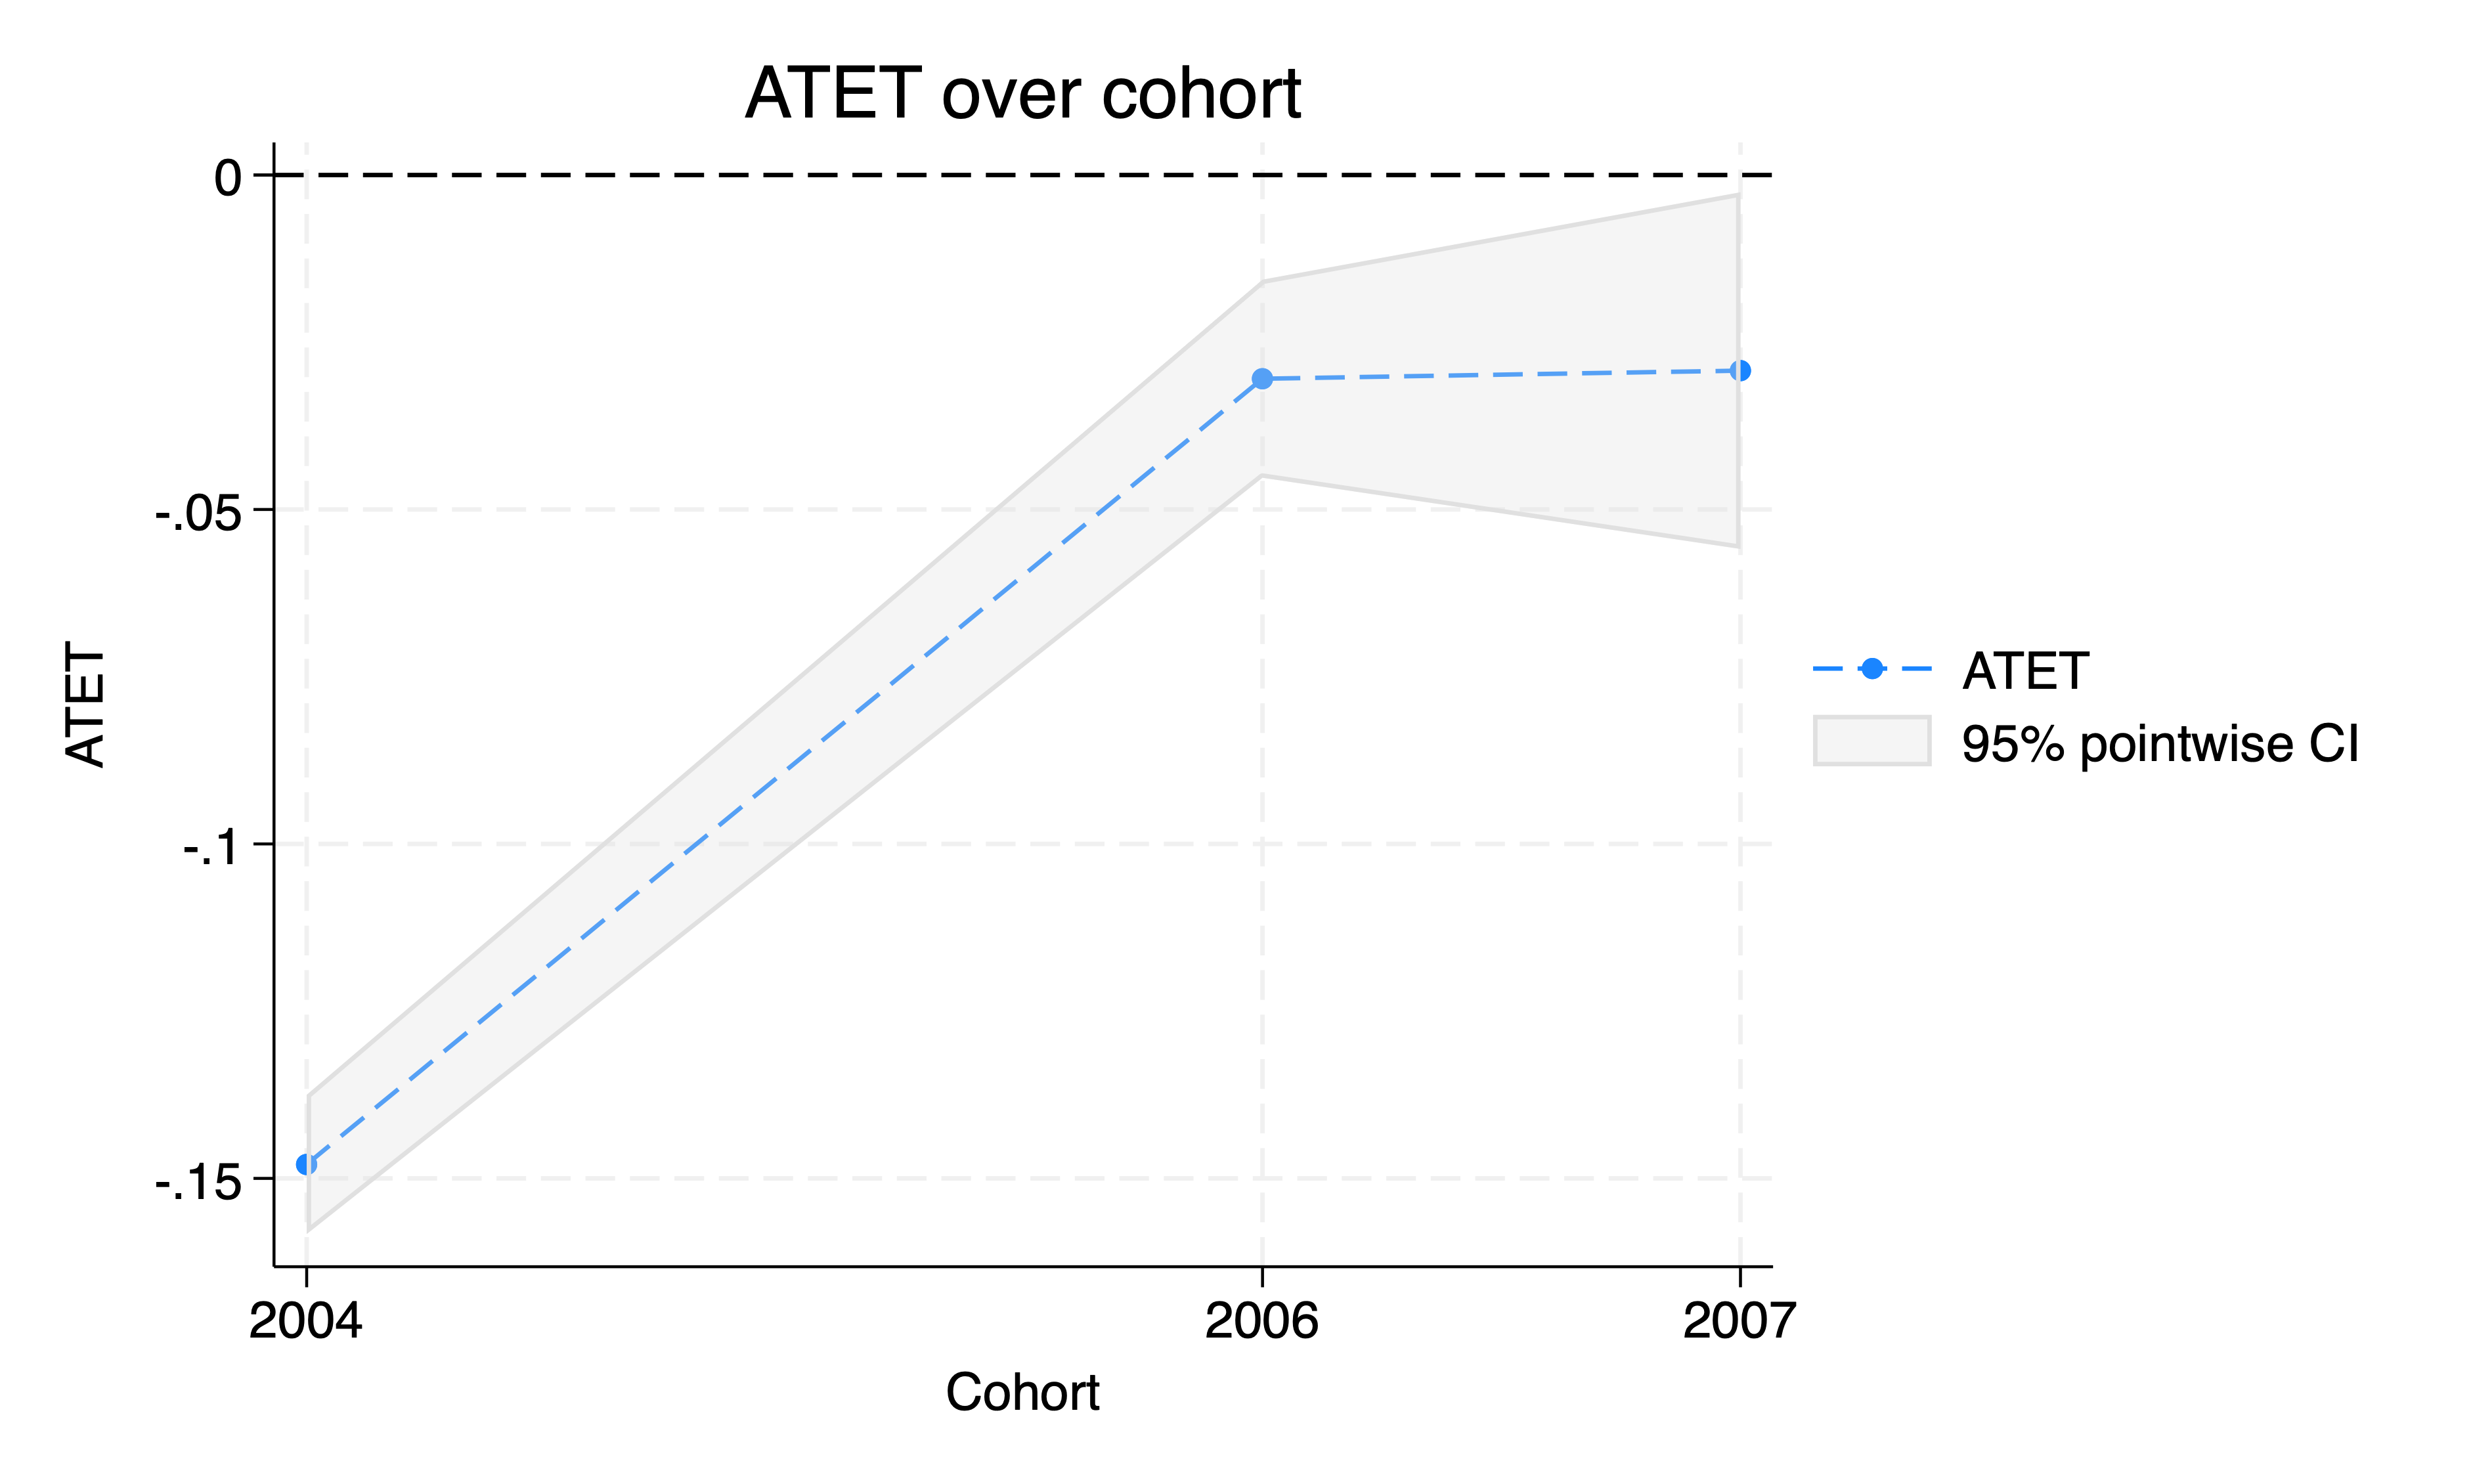
\includegraphics[scale=0.12]{png/c2}
\end{figure}
\end{frame}

%------------------------------------------------------------------------------
\begin{frame}
  \frametitle{ATETs across time}
%------------------------------------------------------------------------------
\begin{align*}
  \theta(\myred{\bf t}) = 
  \sum_{g \in \G} 
  \myred{\I( t \geq g) \Pr(G = g| G \leq t)}
  ATET(g, t)
\end{align*}
\vskip 0.3cm
\begin{itemize}
\item 
\hyperlink{hdid_output.pdf.4}{\tt estat aggregation, weights(cohort) {\bf time}
 \myred{graph}}

 \end{itemize}

\begin{figure}[H]
\centering
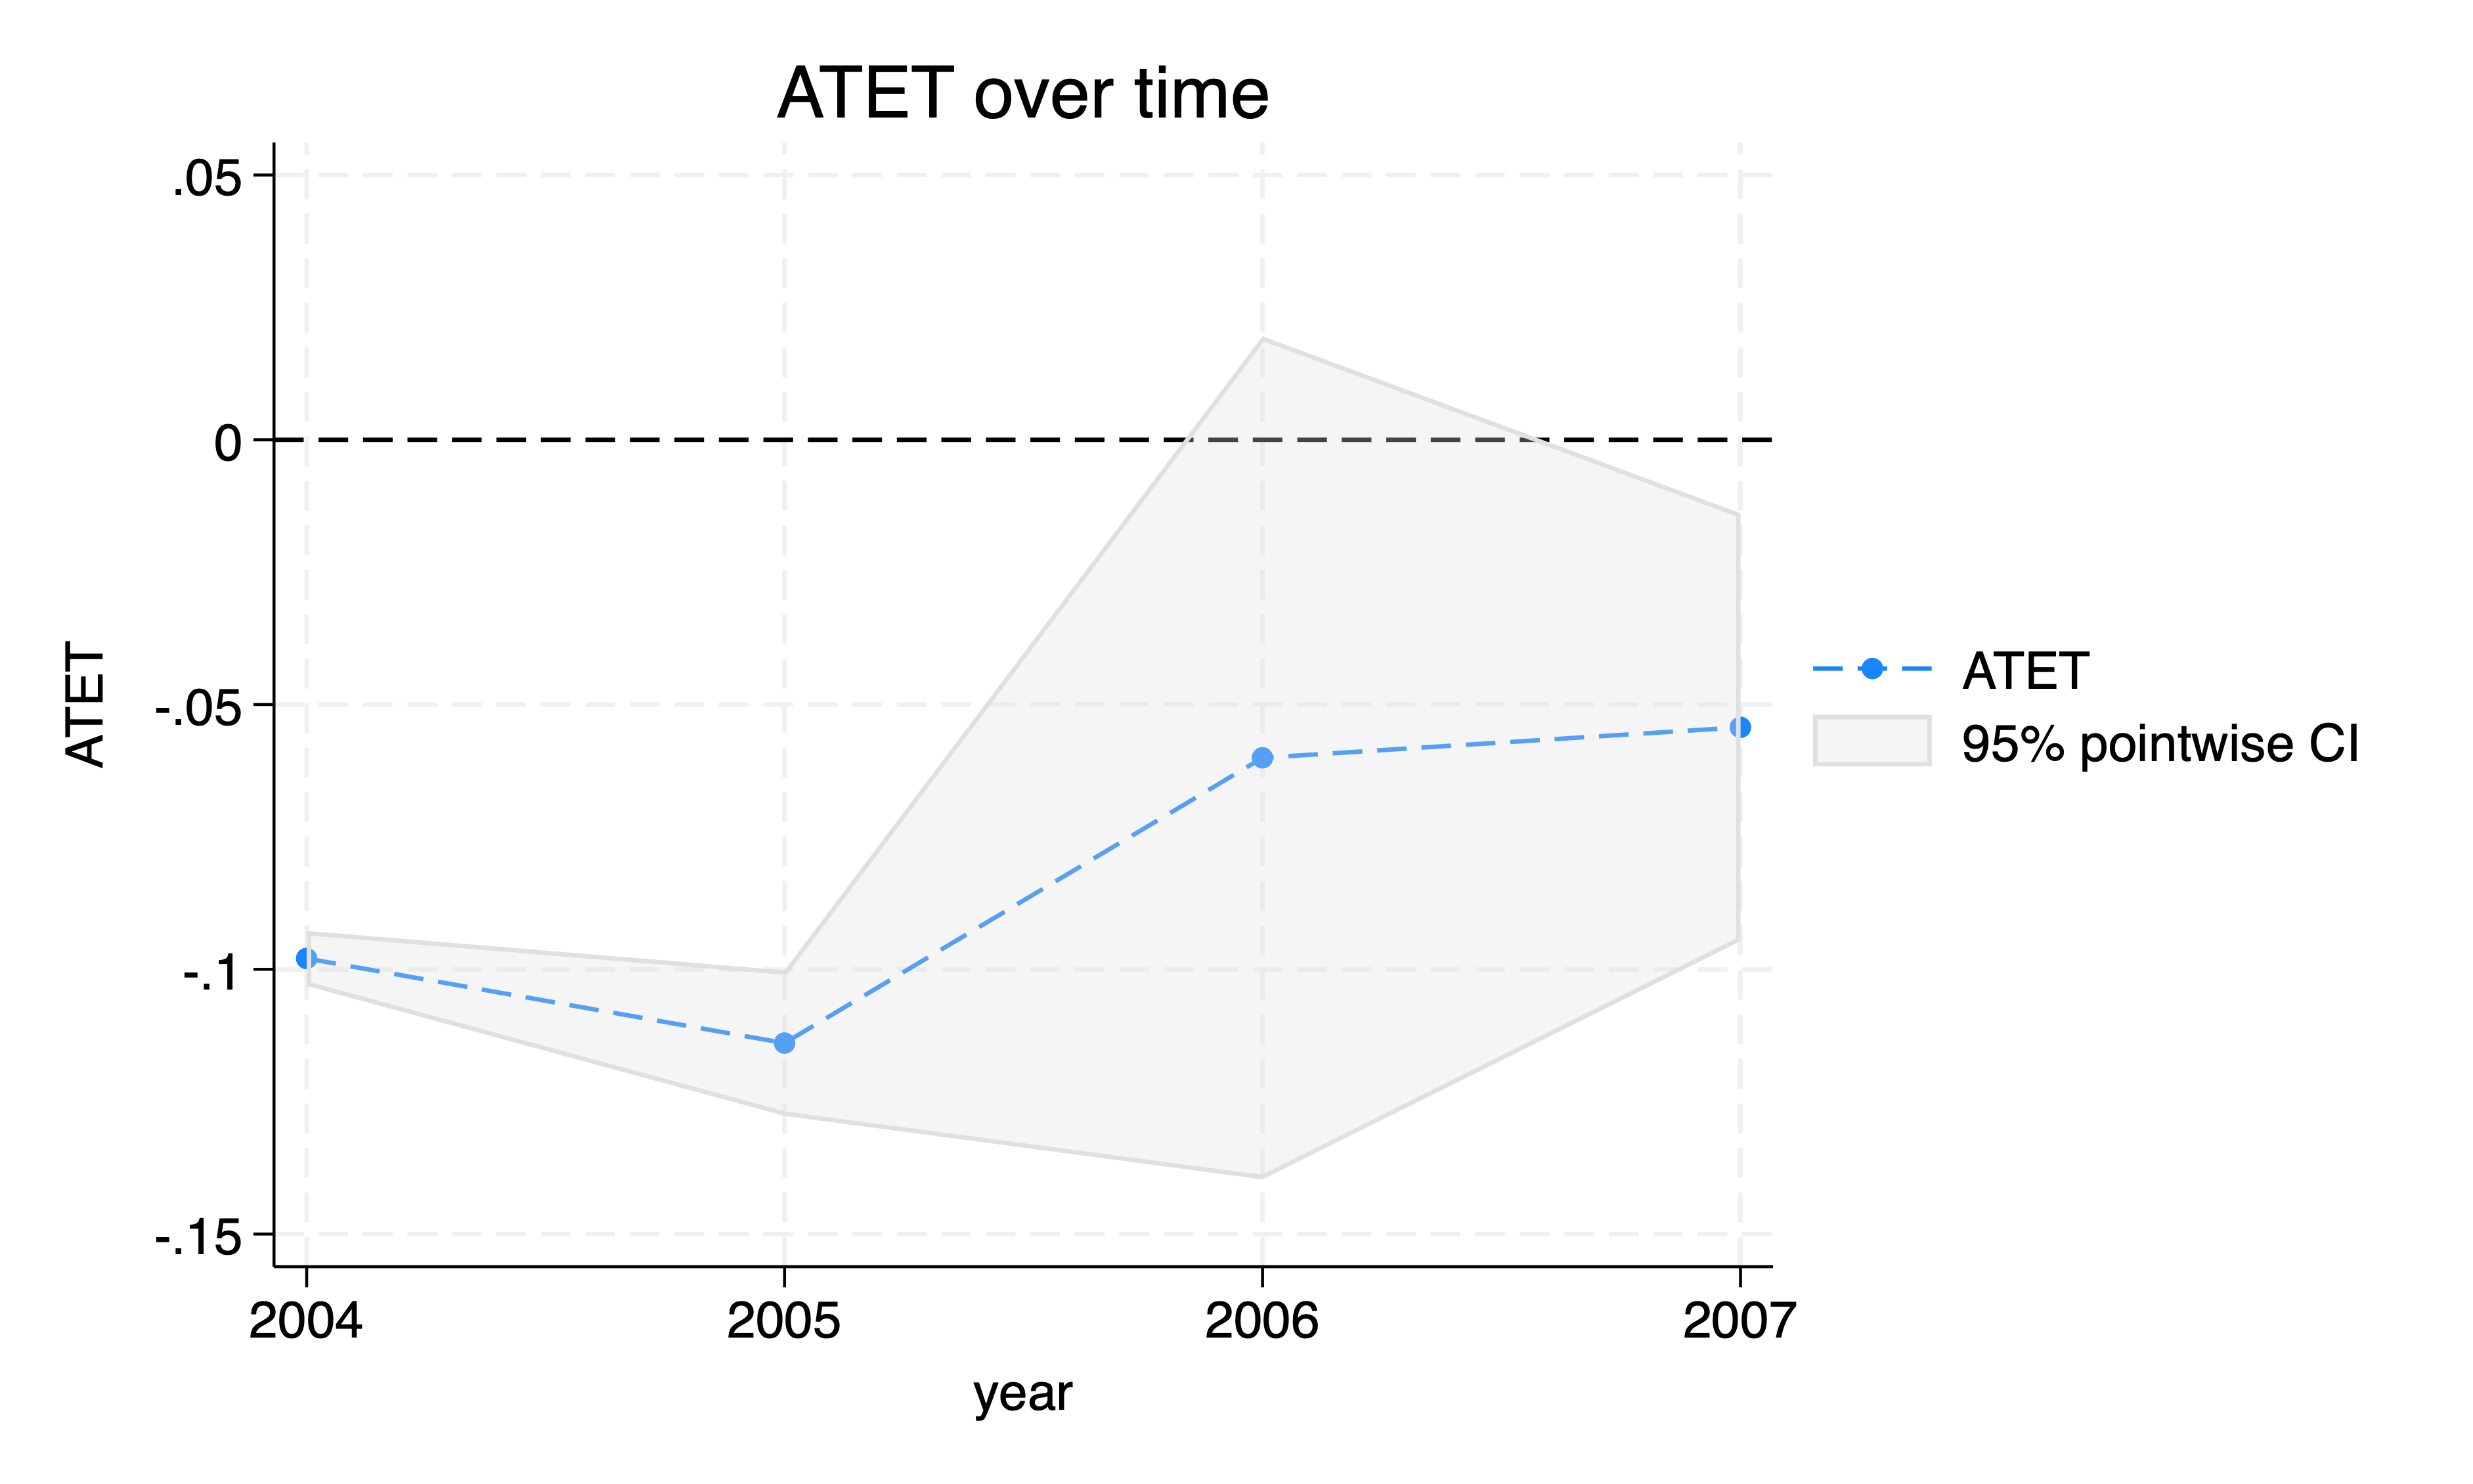
\includegraphics[scale=0.12]{png/t2}
\end{figure}
\end{frame}

%------------------------------------------------------------------------------
\begin{frame}
  \frametitle{Overall aggregations}
%------------------------------------------------------------------------------
\begin{itemize}
\item A single number to summarize ATET's

\begin{align*}
  \theta = \frac{1}{\kappa} \sum_{g\in \G} \sum_{t=2}^T 
  \I (t \geq g) \Pr(G=g | G \leq T) ATET(g,t)
\end{align*}

\item {\tt estat aggregation, weights(cohort) {\bf overall}}
\stlogscaled{0.8}{logs/ex5}

\end{itemize}
\end{frame}

%------------------------------------------------------------------------------
\section{Four estimators}
\begin{frame}
  \frametitle{Potential outcome framework}
%------------------------------------------------------------------------------
Some notations:

\begin{itemize}
\item \myred{$y_{i,t}(g)$} is unit $i$'s \myblue{potential outcome} at
  \myblue{time $t$} if it \myblue{starts treatment} at time \myblue{$g$}

\item \myred{$y_{i,t}(\infty)$} is unit $i$'s \myblue{potential outcome} at
  \myblue{time $t$} if it is \myblue{never treated}

\item \myred{$G_i$} indicates unit $i$'s \myblue{cohort} (when the treatment
  starts), and it is one element
  in $\G = \{2, \ldots, G, \infty\}$

\item \myred{$y_{i,t}$} is unit $i$'s \myblue{observed outcome} at time $t$
  $$
  y_{i,t} = \myred{\underbrace{\I(t < G_i) y_{i, t}(\infty)}_\text{before
  treatment}} 
  + \myblue{\underbrace{\I(t \geq G_i) y_{i,t}(G_i)}_\text{after treatment}}
  $$
\end{itemize}
\end{frame}

%------------------------------------------------------------------------------
\begin{frame}
  \frametitle{Heterogeneous ATETs}
%------------------------------------------------------------------------------
\begin{align*}
  ATET(g, t) = \E[y_{i, t}(g) - y_{i, t}(\infty) | G_i = g]
\end{align*}

Remarks
\begin{itemize}
\item $ATET(g, t)$ is \myred{a function of two arguments}: cohort $g$ and time
  $t$

\item $ATETs$ can be heterogeneous \myred{over cohorts, across time, across
  both time and cohorts} 

\item Objective: consistently \myred{estimate ATETs} and \myred{summarize} them
\end{itemize}
\end{frame}

%------------------------------------------------------------------------------
\begin{frame}
  \frametitle{Key assumptions}
%------------------------------------------------------------------------------
\begin{itemize}
  \item Observe I.I.D samples of $\{y_{i,t}, \xb_{i,t}, \zb_{i,t},
    d_{i,t}\}_{i=1, t=1}^{i=N, t=T}$, where $\xb_{i,t}$ and $\zb_{i,t}$ are
    covariates, and $d_{i,t}$ is observational level treatment indicator

\item No one is treated in the first period

\item No anticipation in pre-treatment periods $t < g$
  $$
  \E[y_{i, t}(g)|\xb, G_i = g]  =  \E[y_{i, t}(\infty)|\xb, G_i=g]
  $$

\item Conditional parallel trend
  $$
  \E[y_{i, t}(\infty) - y_{i, t-1}(\infty)|\xb, G_i = g]  =  
  \E[y_{i, t}(\infty) - y_{i, t-1}(\infty)|\xb, G_i = \infty]  
  $$
\item Overlap assumption for propensity scores
\end{itemize}
\end{frame}

%------------------------------------------------------------------------------
\begin{frame}
\frametitle{Canonical DID}
%------------------------------------------------------------------------------
\begin{figure}[H]
\centering
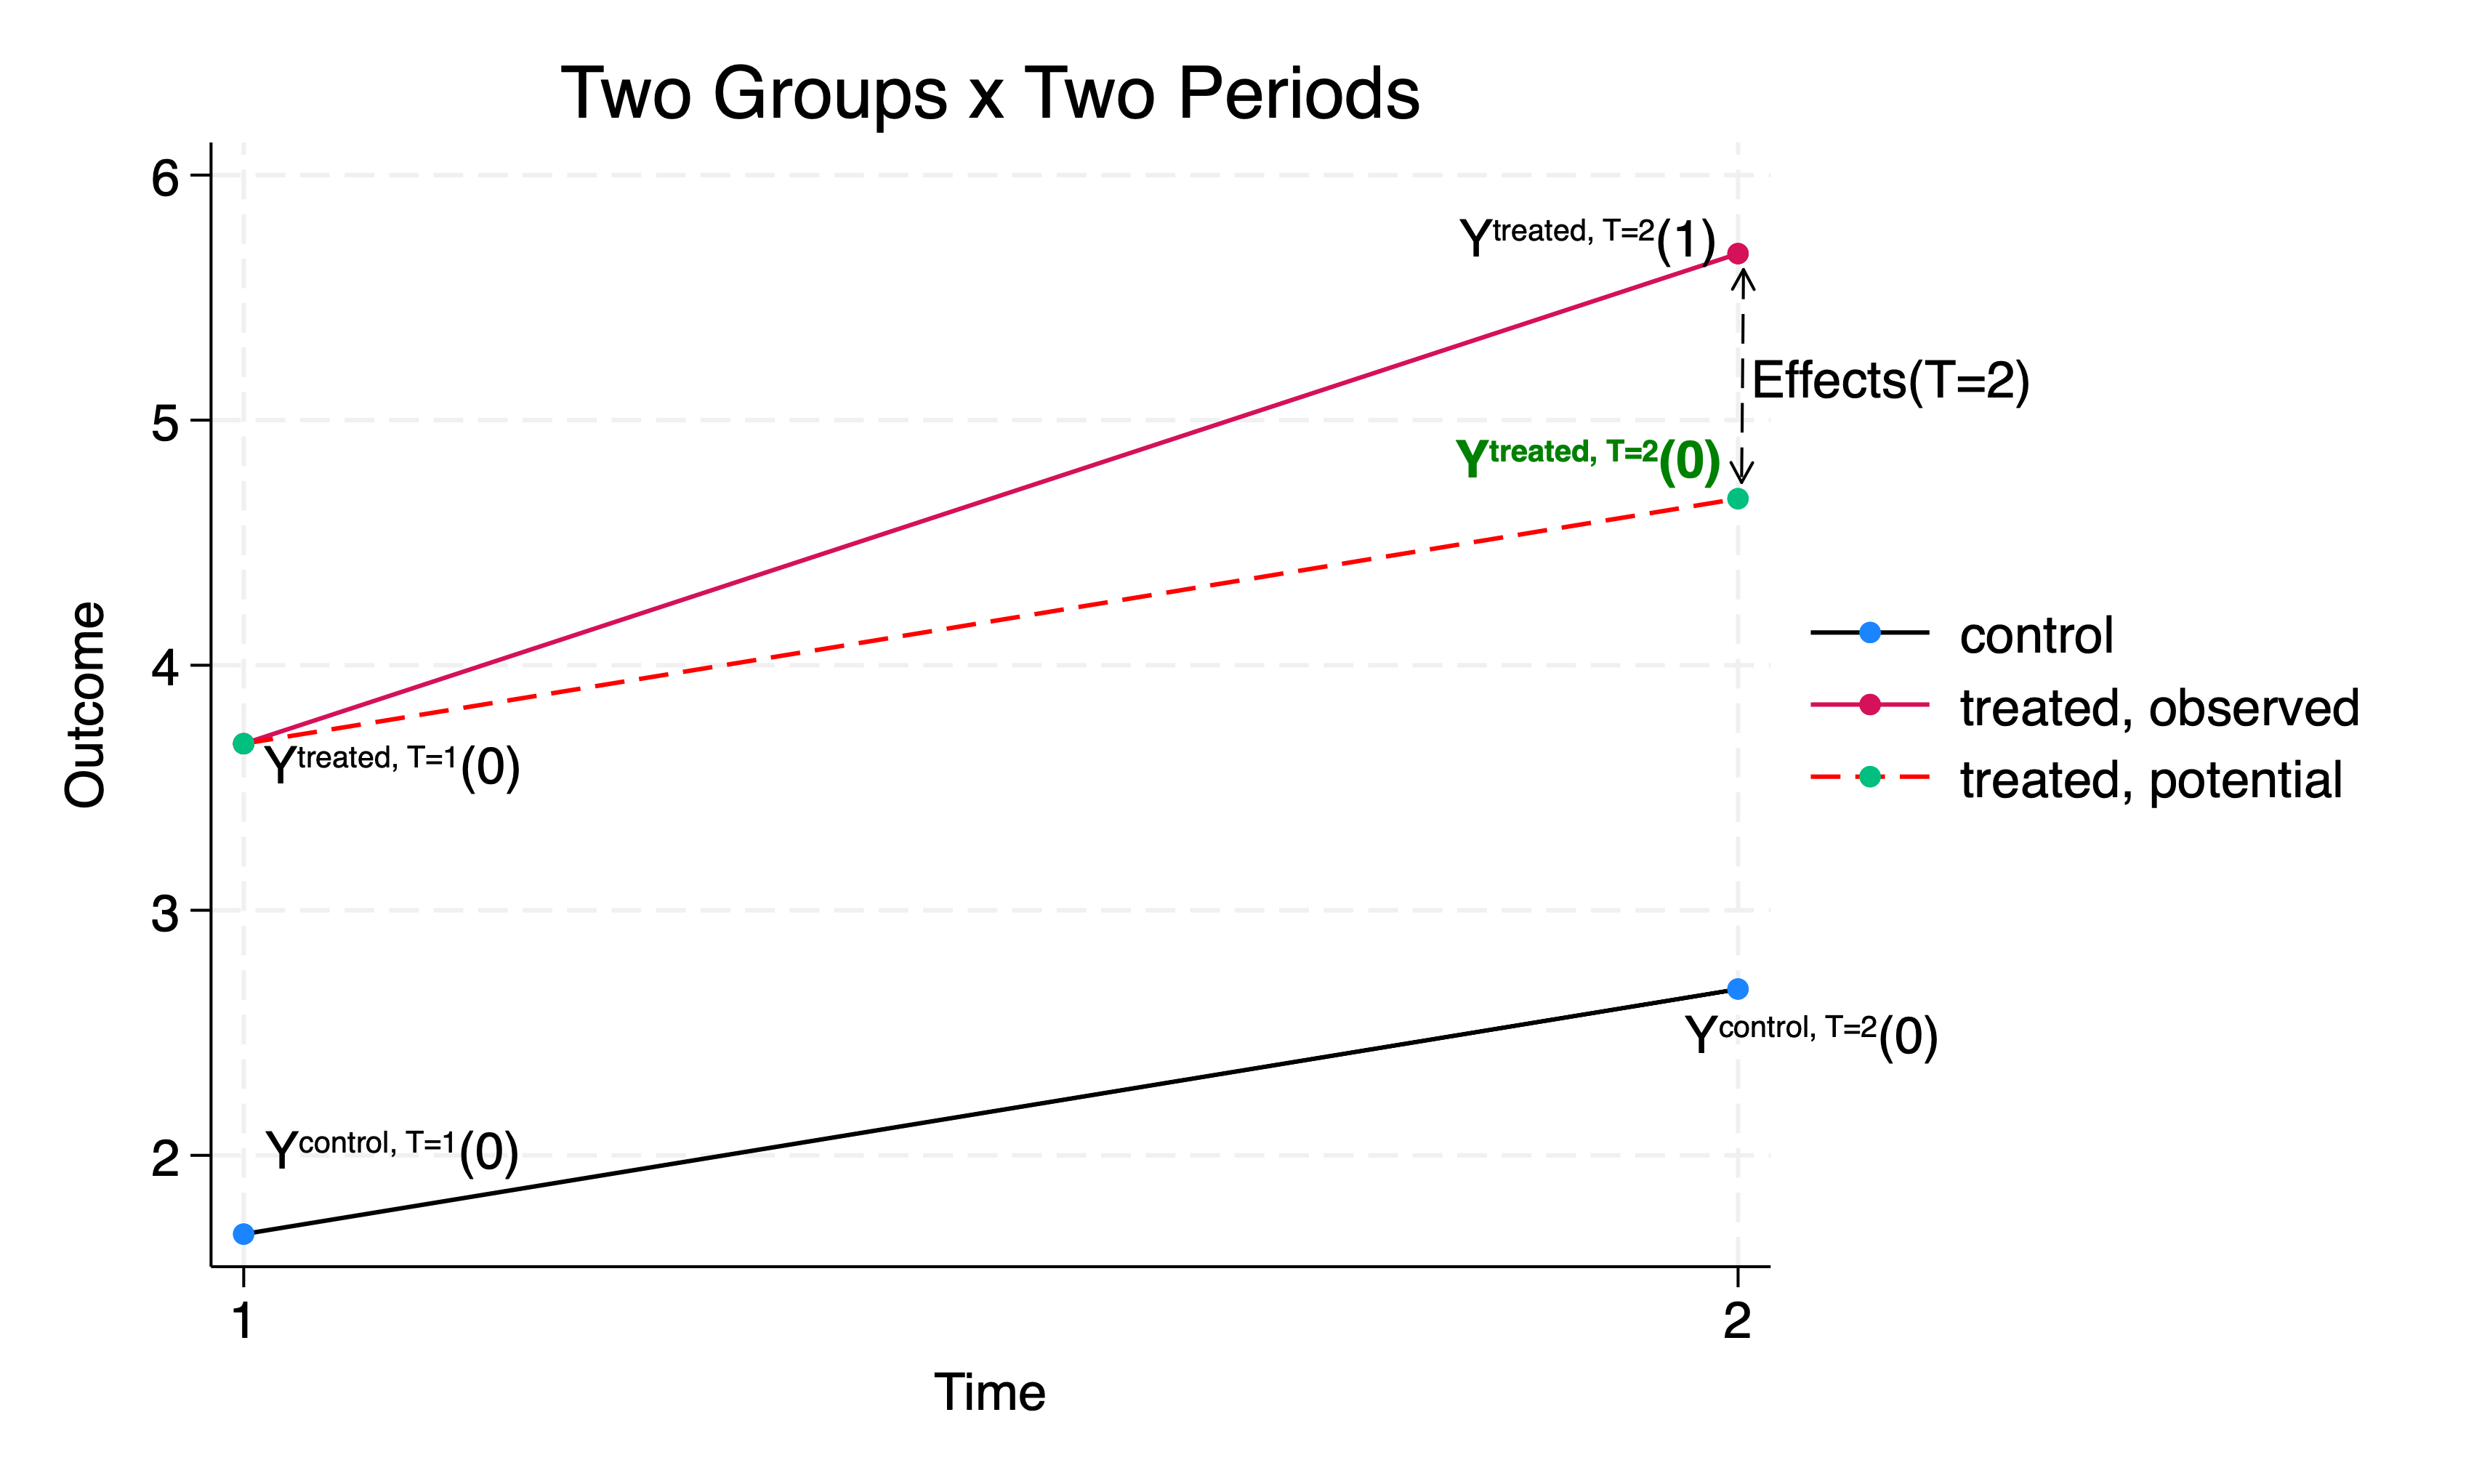
\includegraphics[scale=0.15]{png/did2x2}
\end{figure}

{\small
\begin{align*}
Effects &= \myred{\left[Y^{treated, T=2}(1) - Y^{treated, T=1}(0)\right]}
-
\myblue{\left[ Y^{control, T=2}(0) - Y^{control, T=1}(0) \right]} \\
&= \myred{
\underbrace{\left[Y^{treated, T=2} - Y^{treated, T=1}\right]}
_\text{treated differences}
}
-
\myblue{\underbrace{
\left[ Y^{control, T=2} - Y^{control, T=1} \right]}_\text{untreated differences}
}
\end{align*}
}
\end{frame}


%------------------------------------------------------------------------------
\begin{frame}
\frametitle{Heterogenous DID: benchmark time $g - 1$}
%------------------------------------------------------------------------------
\begin{figure}[H]
\centering
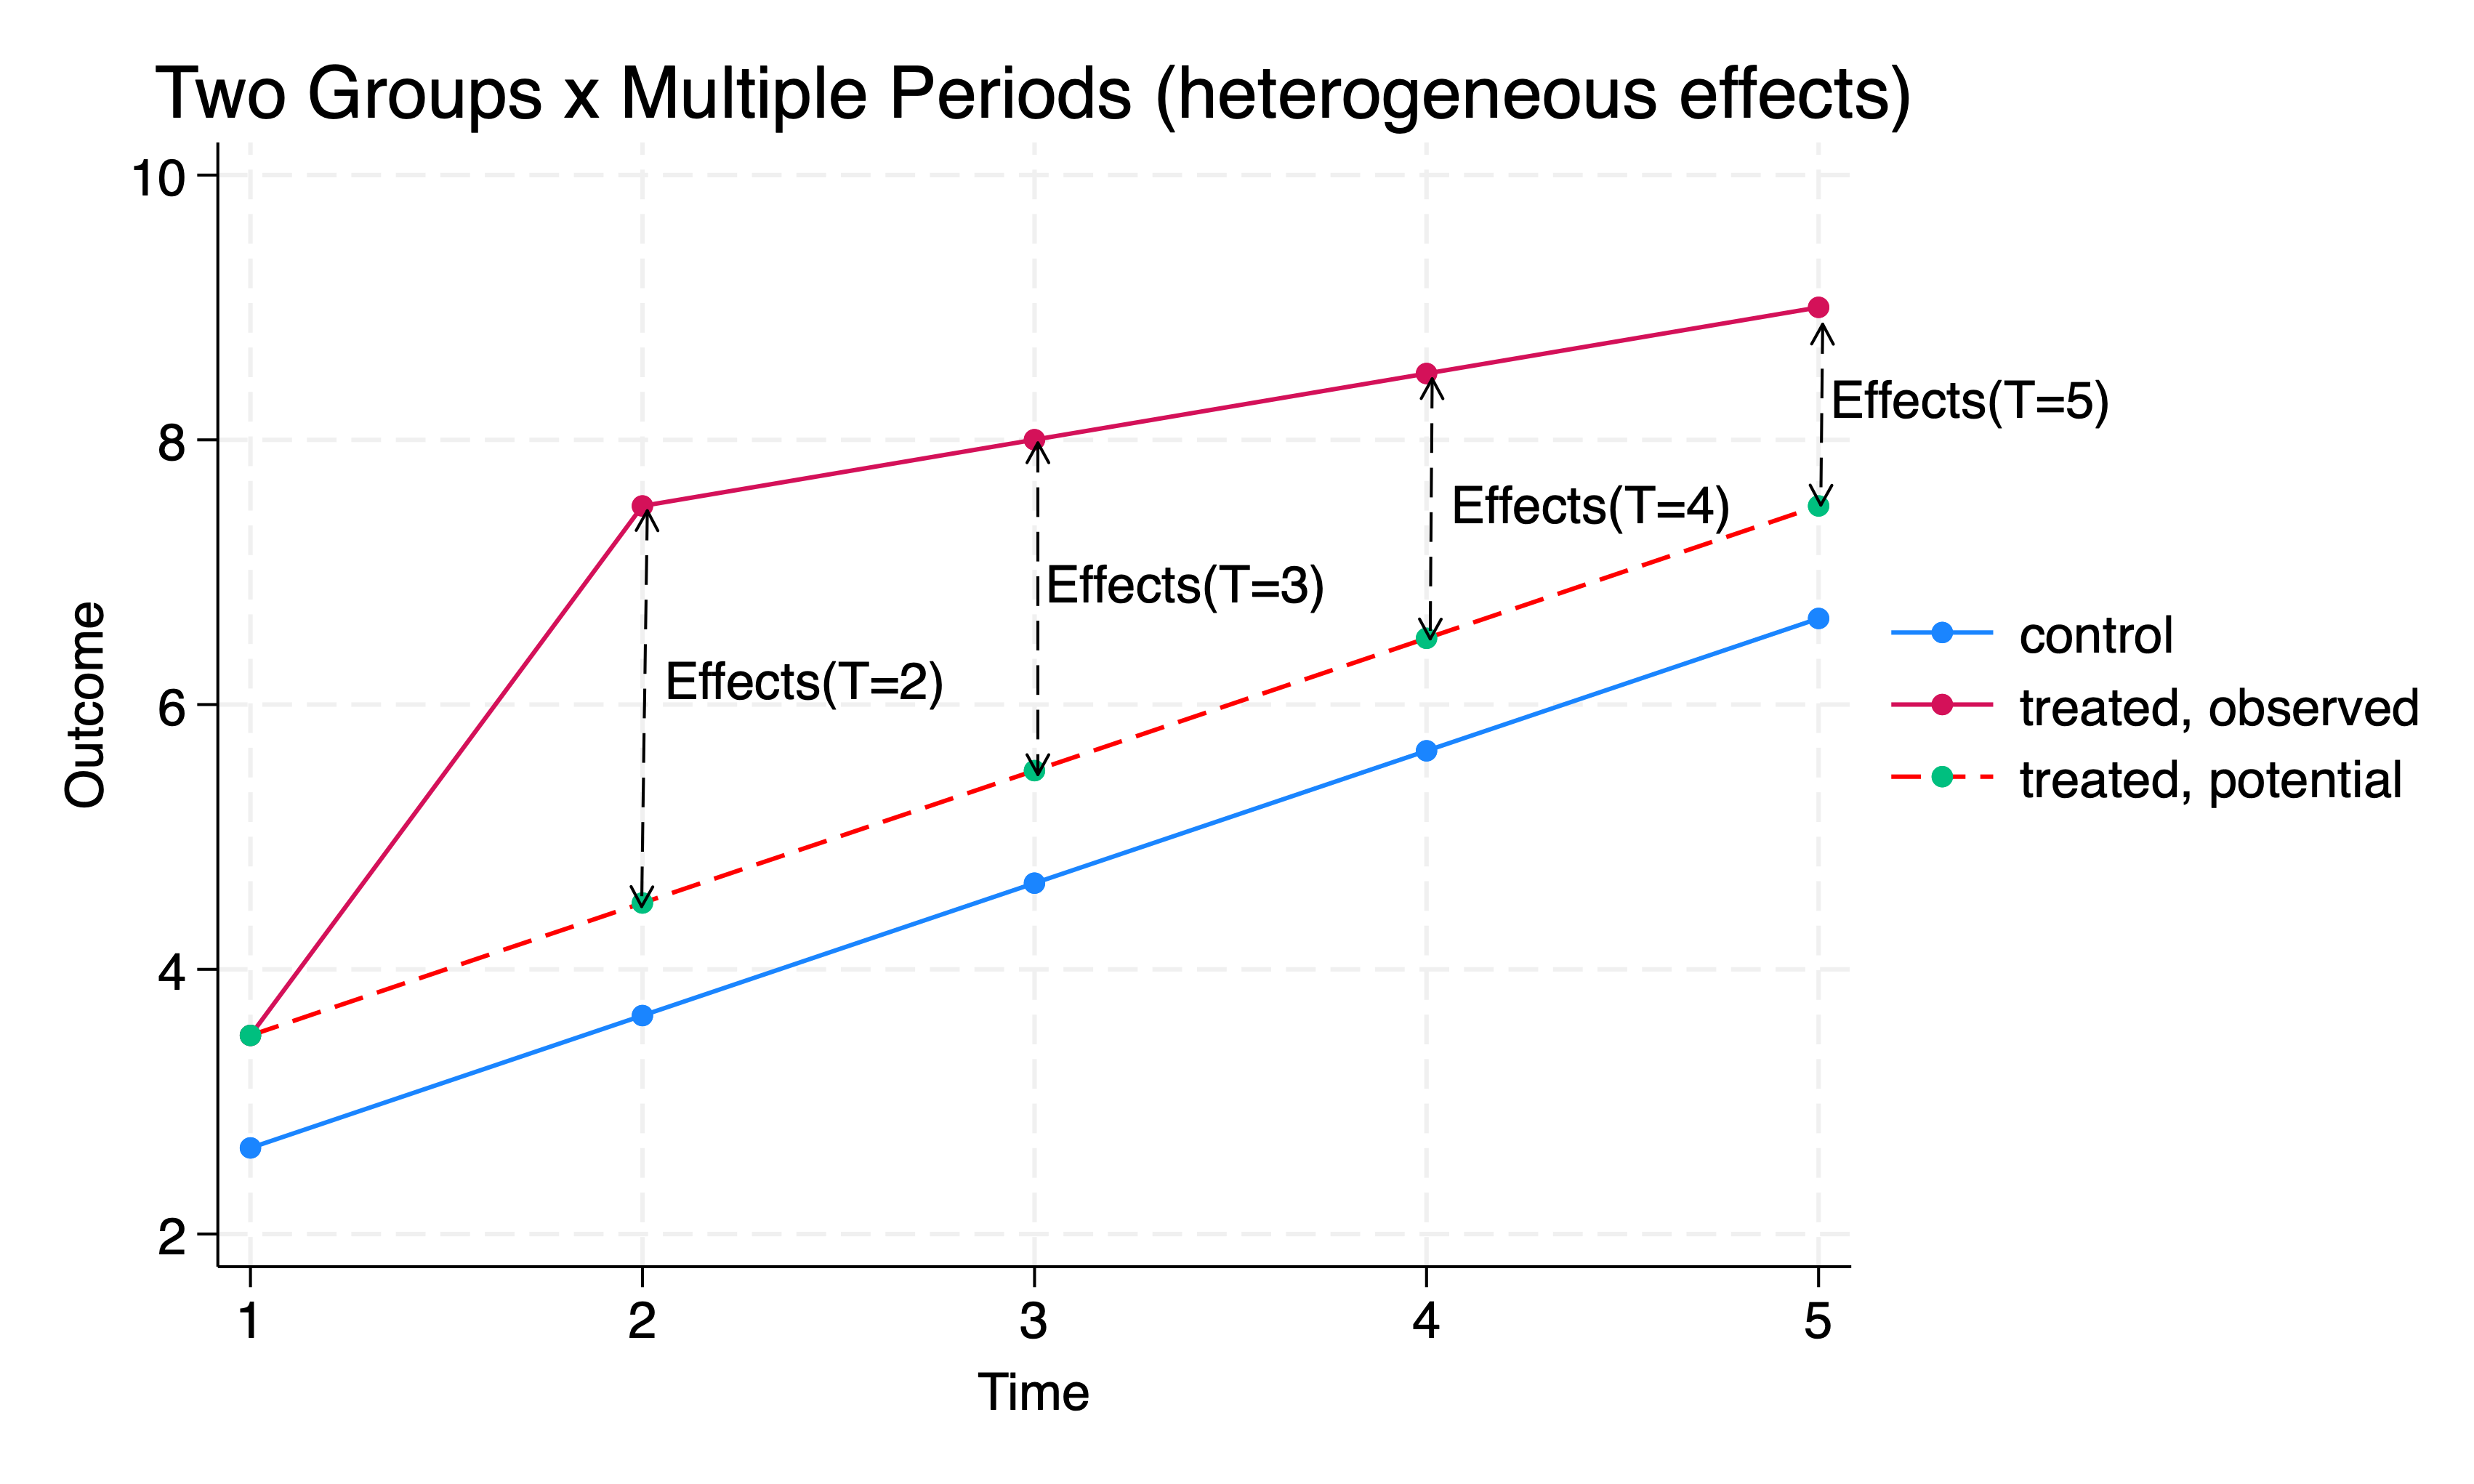
\includegraphics[scale=0.2]{png/did2x5_heter}
\end{figure}
\end{frame}

%------------------------------------------------------------------------------
\begin{frame}
\frametitle{$ATET(g,t)$ is reduced to $2 \times 2$ DID}
%------------------------------------------------------------------------------
\begin{figure}[H]
\centering
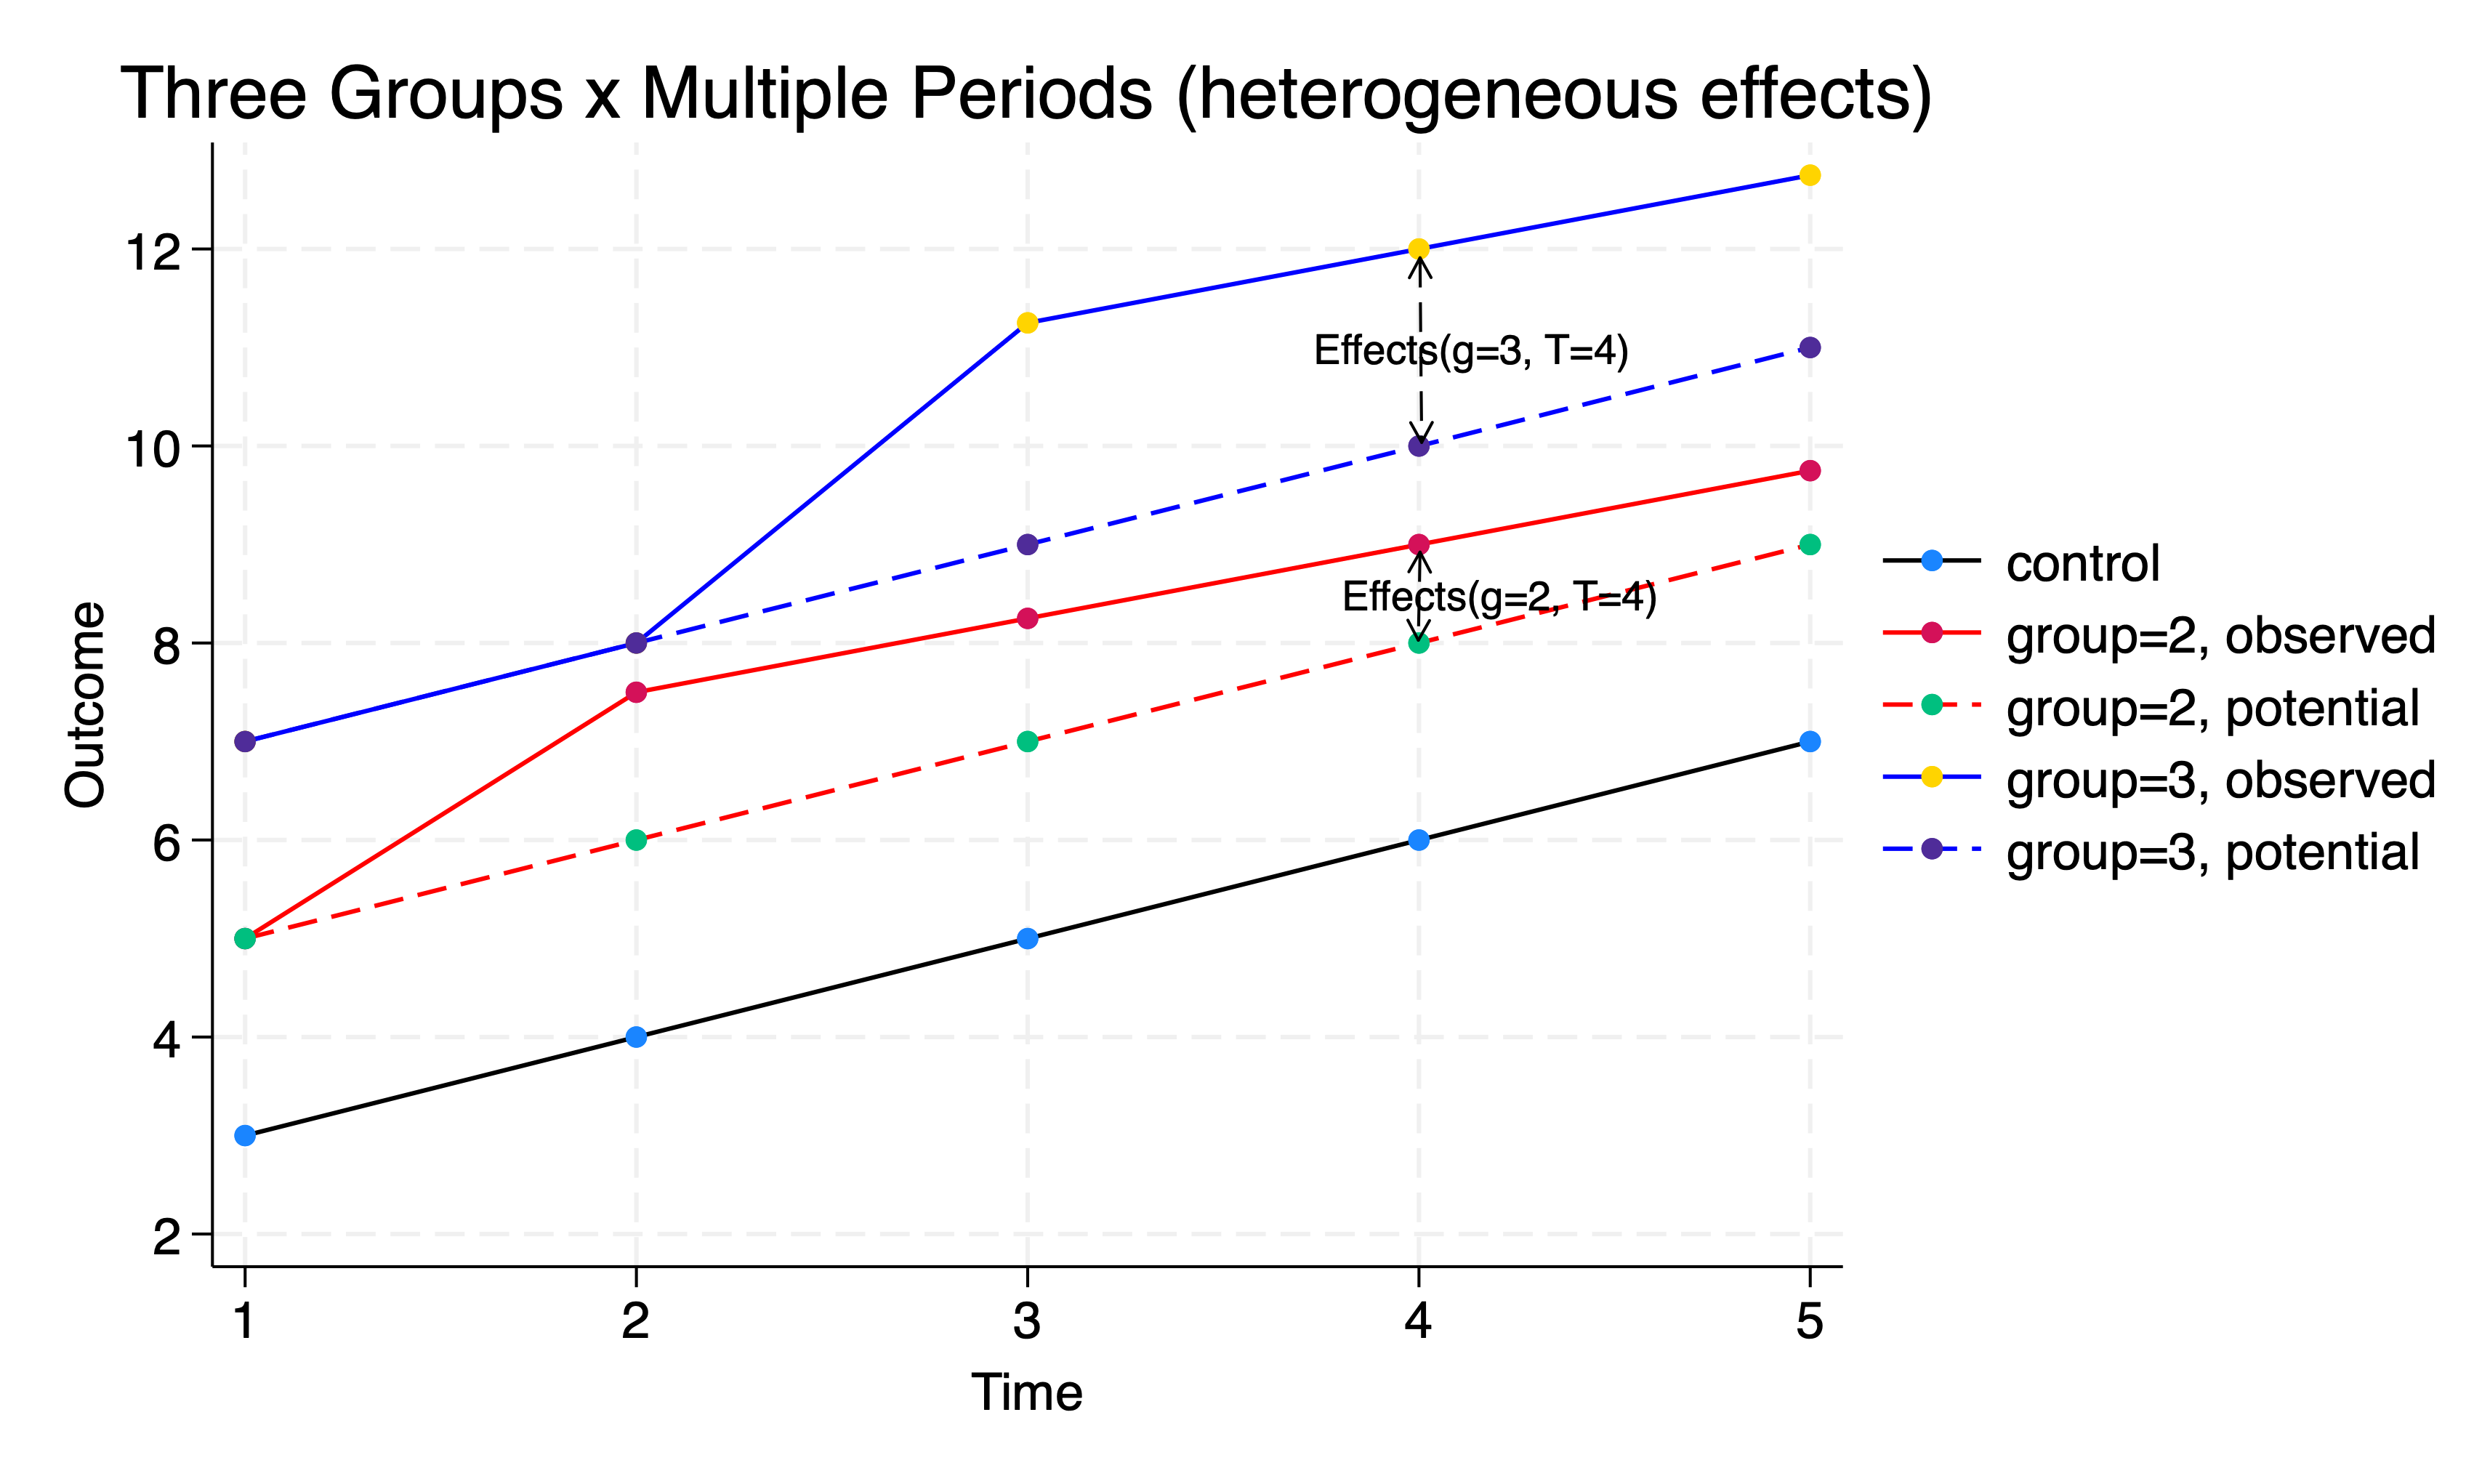
\includegraphics[scale=0.2]{png/did3x5_heter}
\end{figure}
\end{frame}


%------------------------------------------------------------------------------
\begin{frame}
  \frametitle{Regression adjustment (RA)}
%------------------------------------------------------------------------------

\begin{align*}
  ATET(g, t) &=
  \E\left[
    \frac{K_g}{\E(K_g)} 
    \left(
    y_t - y_{g - 1} - m_{g, t}
    \right)
  \right] \\
  &= \myred{\underbrace{\E\left[ y_t - y_{g - 1} | K_g = 1 \right]}_\text{treated
  differences}}
  - \myblue{\underbrace{\E\left[ m_{g, t}(\xb) | K_g = 1 \right]}_\text{untreated
  differences}}
\end{align*}
where
\begin{itemize}
\item $K_g = \I(G_i = g)$ and $m_{g, t}(\xb) = \E (y_t - y_{g-1} | \xb,
    G_i=\infty)$
\item It is $2 \times 2$ difference-in-differences (two groups $\times$ two
  periods)
\item Benchmark time: one period before treatment ($g-1$)
\item Benchmark group: never-treated group ($G_i = \infty$)
\end{itemize}

\vskip 0.5cm
In Stata, we type
\begin{itemize}
\item {\large \tt xthdidregress \myred{ra} 
  \myblue{$\underbrace{(y \quad \xb)}_{m_{g,t}(\xb)}$} (d), group(id)}
\end{itemize}
\end{frame}

%------------------------------------------------------------------------------
\begin{frame}
  \frametitle{Inverse probability weighting (IPW)}
%------------------------------------------------------------------------------
\begin{align*}
  ATET(g, t) = 
  \E\left[
    \left(
    \frac{K_g}{\E(K_g)} 
    - \frac{\frac{p_g(\zb)K_\infty}{1-p_g(\zb)}}
    {\E\left[ \frac{p_g(\zb)K_\infty}{1-p_g(\zb)} \right]}
    \right)
    (Y_t - Y_{g - 1})
  \right]
\end{align*}
where 
\begin{itemize}
  \item $\myred{p_g(\zb) = \Pr(K_g = 1 | \zb, K_g + K_\infty = 1)} = 
\frac{\Pr(K_g = 1| \zb)}{\Pr(K_g + K_\infty = 1 | \zb)}$

\item $\frac{p_g(\zb)}{1 - p_g(\zb)} = \frac{\Pr(K_g =1
  |\zb)}{\Pr(K_\infty=1|\zb)}$. 
  Thus, in the benchmark group (never treated), attach more weights to
  observations that are more probably observed in the cohort $g$

\item We estimate $p_g(\zb)$ by a logit regression
\end{itemize}

\vskip 0.5cm
In Stata, we type
\begin{itemize}
\item {\large \tt xthdidregress \myred{ipw} 
  (y) \myblue{$\underbrace{(d\ \zb)}_{p_g(\zb)}$}, group(id)}
\end{itemize}
\end{frame}

%------------------------------------------------------------------------------
\begin{frame}
  \frametitle{Augmented inverse probability weighting (AIPW)}
%------------------------------------------------------------------------------
\begin{align*}
  ATET(g, t) &= 
  \E\left[
    \myblue{\underbrace{
    \left(
    \frac{K_g}{\E(K_g)} 
    - \frac{\frac{p_g(\zb)K_\infty}{1-p_g(\zb)}}
    {\E\left[ \frac{p_g(\zb)K_\infty}{1-p_g(\zb)} \right]}
    \right)
    (
    Y_t - Y_{g - 1}}_\text{IPW}} - \myred{\overbrace{m_{g,
    t}(\xb)}^\text{augmented term}}
    )
  \right] 
\end{align*}
\begin{itemize}
  \item AIPW is \myred{doubly robust}: only one of the outcome model or the
    treatment model needs to be correctly specified
\end{itemize}

\vskip 0.5cm
In Stata, we type
\begin{itemize}
\item {\large \tt xthdidregress \myred{aipw} 
  \myred{$\underbrace{(y\ \xb)}_{m_{g,t}(\xb)}$} 
  \myblue{$\underbrace{(d\ \zb)}_{p_g(\zb)}$}, 
group(id)}
\end{itemize}
\end{frame}

%------------------------------------------------------------------------------
\begin{frame}
  \frametitle{TWFE}
%------------------------------------------------------------------------------
Traditional TWFE:
$$
y_{it} = \theta_t + \eta_i +  \myred{d_{it} \alpha} + v_{it}
$$


\vskip 1cm
TWFE in \cite{Wooldridge2021}:
$$
	y_{it} = \theta_t + \eta_i +
	\myblue{\sum_{g\in\G}\sum_{s=g}^T\alpha_{g,t} \I(G_i = g, t = s)}
	+ v_{it}
$$
With covariates $\xb$, add full interactions with $\theta_t$, $\eta_i$, and
$\I(G_i =g, t= s)$. 

\vskip 0.5cm
In Stata, we type
\begin{itemize}
\item {\large \tt xthdidregress \myred{twfe} 
  \myred{$\underbrace{(y\ \xb)}_{TWFE \ outcome}$} 
  (d), group(id)}
\end{itemize}
\end{frame}

%------------------------------------------------------------------------------
\begin{frame}
\frametitle{Summary}
%------------------------------------------------------------------------------
\begin{itemize}
    \setlength\itemsep{1em}
\item We illustrate the heterogeneous treatment effects across time and groups
\item Traditional TWFE is inconsistent 
\item {\tt xthdidregress} and {\tt hdidregress} implements four estimators to
remedy the heterogeneity issues
\item {\tt estat atetplot} visualize the heterogeneity at the group-time level
\item {\tt estat aggregation} estimate and visualize the heterogeneity at a 
higher level 
\end{itemize}
\end{frame}

%------------------------------------------------------------------------------
\begin{frame}
\frametitle{Some extensions}
%------------------------------------------------------------------------------
\begin{itemize}
  \item Switchers: treatments are on and off \citep{Chaise2020}
\item Partial identification: event study when parallel trends assumption is
  violated \citep{Rambachan2023}
\item High-dimensional controls: AIPW estimator is Neyman orthogonal
  \citep{Callaway2023}
\end{itemize}
\end{frame}




%------------------------------------------------------------------------------
% reference
\clearpage
{\bf References}
%------------------------------------------------------------------------------
\bibliographystyle{sjlatex/sj}
\bibliography{mybib}

{
\beamertemplatenavigationsymbolsempty
\setbeamercolor{background canvas}{bg=}
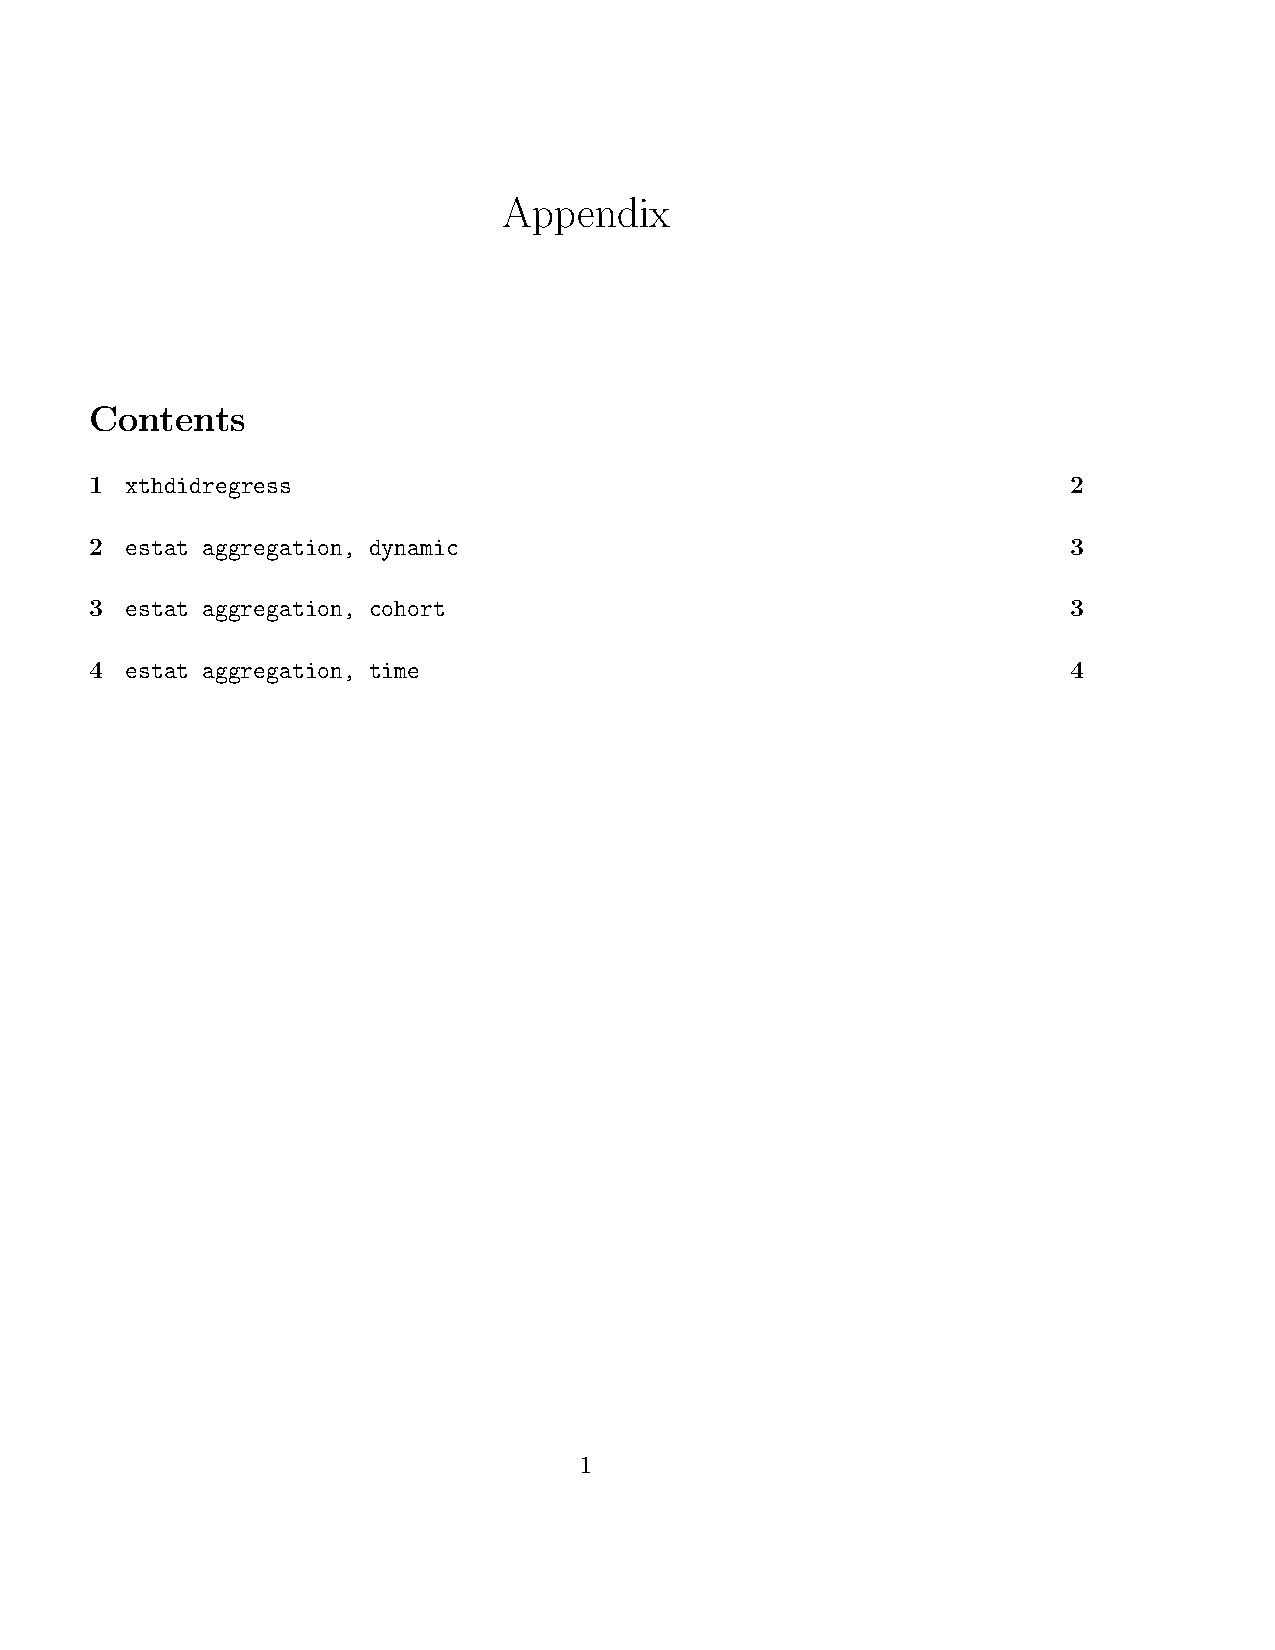
\includepdf[pages=1-4, link=true,fitpaper]{hdid_output.pdf}
}

\end{document}

